\documentclass[compress]{beamer}

\usepackage{graphicx,epstopdf,subfigure,booktabs,natbib,verse}
\usepackage{amsmath,amssymb,amsthm}
\newcommand{\attrib}[1]{% 
\nopagebreak{\raggedleft\footnotesize #1\par}}

%\usetheme[compress,subsection=F]{Singapore}
\useoutertheme[subsection=false]{miniframes}
\useinnertheme{default}
\usecolortheme{seagull}

\bibliographystyle{plainnat}
\bibpunct{[}{]}{;}{a}{}{,}

\usepackage{tikz}
\usetikzlibrary{shapes,arrows,calc,through,backgrounds,shapes.symbols,positioning}


%\usepackage{fourier}

% for themes, etc.

% these will be used later in the title page
\title{Unstructured adaptive mesh generation and sparse matrix storage applied to Stokes flow around cylinders}
%\subtitle{SUBTITLE}
\author{Cameron Bracken\footnote{Humboldt State University}}
\date{E521\\May 1, 2008}


\newcommand{\p}{\partial}


\begin{document}

%%%%%%%%%%%%%%%%%%%%%%%%%%%%%%%%%%%%%%
\begin{frame}
\titlepage
\end{frame}
%%%%%%%%%%%%%%%%%%%%%%%%%%%%%%%%%%%%%%

%%%%%%%%%%%%%%%%%%%%%%%%%%%%%%%%%%%%%%
\begin{frame}{Project Goals}
\begin{enumerate}
\item Solve the 2D Steady Stokes equations via finite elements
\item Investigate the placement of cylindrical obstructions in the flow field
\item Adaptively generate the finite element mesh
\item Utilize sparse matrix storage
\end{enumerate}
\end{frame}
%%%%%%%%%%%%%%%%%%%%%%%%%%%%%%%%%%%%%%

\section{Introduction}
%%%%%%%%%%%%%%%%%%%%%%%%%%%%%%%%%%%%%%
%\subsection{In The Beginning}
%\begin{frame}{In The Beginning}
%\pause
%\poemtitle{In the beginning} 
%\settowidth{\versewidth}{And objects at rest tended to remain at rest} 
%\begin{verse}[\versewidth] 
%Then Newton was born, \\* 
%And objects at rest tended to remain at rest, \\* 
%And objects in motion tended to remain in motion, \\* 
%And energy was conserved 
%and momentum was conserved 
%and matter was conserved \\* 
%And it was pretty darn conservative. 
%\end{verse} 
%\attrib{Possibly from \textit{Analog}, circa 1950}
%\begin{flushright}{\footnotesize [Edited for PCness by Cameron]}\end{flushright}
%\end{frame}
%%%%%%%%%%%%%%%%%%%%%%%%%%%%%%%%%%%%%%

%%%%%%%%%%%%%%%%%%%%%%%%%%%%%%%%%%%%%%
%\section{Background}
%\subsection{The Equations}
%\begin{frame}{Navier-Stokes equations}
%Represent conservation of momentum of a fluid.
%\begin{equation}
%  \rho {\bf V}_t - \mu \nabla^2 {\bf V} + \rho ({\bf V}  \cdot \nabla ) {\bf V} 
%    + \nabla p = 0 \label{eqn:ns}
%\end{equation}
%\pause
%And along with the continuity equation
%\begin{equation}
%\rho_t + \nabla \cdot (\rho \mathbf{V}) = 0.
%\end{equation}
%We have enough information to describe any fluid...\pause that is  isothermal, \pause pure, \pause  not under the influence of electromagnetic forces, \pause or in the subsurface!
%\end{frame}
%%%%%%%%%%%%%%%%%%%%%%%%%%%%%%%%%%%%%%

%%%%%%%%%%%%%%%%%%%%%%%%%%%%%%%%%%%%%%
\subsection{Stokes equations - What I did solve}
\begin{frame}{Stokes equations - Simplification}
\pause
Start with the NS equations:
$$\rho {\bf V}_t - \mu \nabla^2 {\bf V} + \rho ({\bf V}  \cdot \nabla ) {\bf V} 
    + \nabla p = 0 \label{eqn:ns}$$
    \pause
Assume steady,
$$\mu\nabla^2 {\bf V} + \rho ({\bf V}  \cdot \nabla ) {\bf V} + \nabla p = 0 \label{eqn:ns}$$
    \pause
Assume irrotational flow,
\begin{equation}\nu\nabla^2 \mathbf {V} + \nabla p = 0%\tag{Stokes Equations}
\end{equation}
And we arrive at the \alert{Stokes equations}.\\\pause
And for the continuity equation, assume incompressible,
    \pause
\begin{equation}\nabla \cdot\mathbf{V} = 0%\tag{Continuity}
\end{equation}
We have enough information to describe any \alert{very} viscous and/or slow moving fluid ($RE\ll 1$,creeping flow).
\end{frame}

%%%%%%%%%%%%%%%%%%%%%%%%%%%%%%%%%%%%%%%
\subsection{Problem Statement}
\begin{frame}{Formal Problem Statement}
\begin{columns}
\begin{column}{0.5\textwidth}
Scalar Equations:
$$- \nu \frac{\p^2 u}{\p x^2} - \nu \frac{\p^2 u}{\p y^2} + \frac{\p p}{\p x}  = 0$$
$$- \nu \frac{\p^2 v}{\p x^2} - \nu \frac{\p^2 v}{\p y^2}+ \frac{\p p}{\p y}  = 0 $$
$$\frac{\p u}{\p x} + \frac{\p v}{\p y} = 0$$
\end{column}
\begin{column}{0.5\textwidth}
\pause
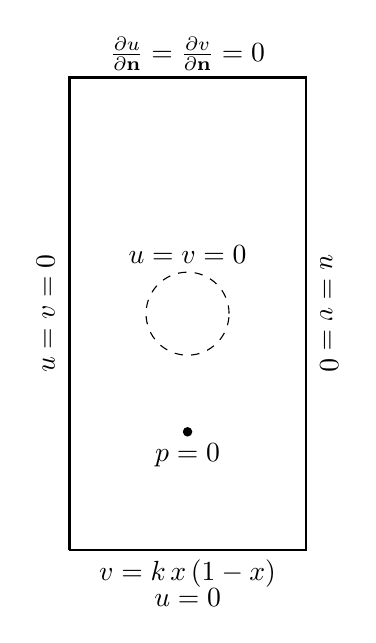
\begin{tikzpicture}[scale=3]
	\draw[thick](0,0)--(0,2)--(1,2)--(1,0)--(0,0);
	
	\draw (.5,2.1) node{$\frac{\p u}{\p \mathbf{n}}=\frac{\p v}{\p \mathbf{n}}=0$};
	\draw (.5,-.1) node{$v=k\,x\,(1-x)$};
	\draw (.5,-.2) node{$u=0$};
	\draw (-.1,1) node[rotate=90]{$u=v=0$};
	\draw (1.1,1) node[rotate=-90]{$u=v=0$};
	\draw[style=dashed] (.5,1) circle(5pt);
	\draw (.5,1.25) node{$u=v=0$};
	\filldraw [black] 
		(.5,.5) circle (.5pt);
	\draw (.5,.4) node{$p=0$};
	
\end{tikzpicture}
\end{column}
\end{columns}
\end{frame}
%%%%%%%%%%%%%%%%%%%%%%%%%%%%%%%%%%%%%%

%%%%%%%%%%%%%%%%%%%%%%%%%%%%%%%%%%%%%%
\begin{frame}{Basis Functions}
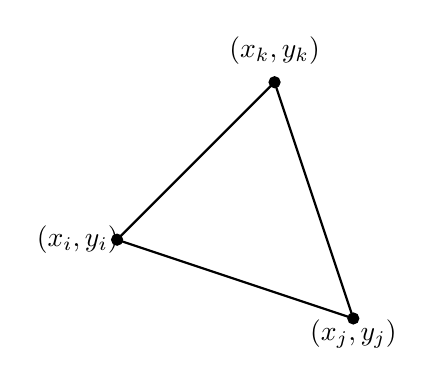
\begin{tikzpicture}[scale=2]
	\draw[thick](0,0)--(1,1)--(1.5,-.5)--(0,0);
	
	\filldraw [black] (0,0) circle (1pt) 
				(1,1) circle (1pt) 
				(1.5,-.5) circle (1pt);
				
	\draw (-.25,0) node{$(x_i,y_i)$};
	\draw (1.5,-.6) node{$(x_j,y_j)$};
	\draw (1,1.2) node{$(x_k,y_k)$};
\end{tikzpicture}
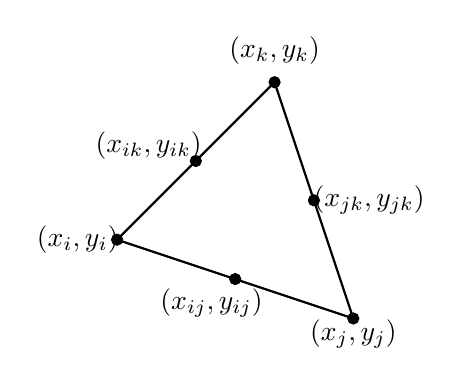
\begin{tikzpicture}[scale=2]
	\draw[thick]
		(0,0)--(1,1)--(1.5,-.5)--(0,0);
	\filldraw [black] 
		(0,0) circle (1pt) 
		(1,1) circle (1pt) 
		(1.5,-.5) circle (1pt)
		(.5,.5) circle (1pt) 
		(.75,-.25) circle (1pt) 
		(1.25,.25) circle (1pt);		
	\draw 
		(-.25,0) node{$(x_i,y_i)$}
		(1.5,-.6) node{$(x_j,y_j)$}
		(1,1.2) node{$(x_k,y_k)$}
		(.2,.6) node{$(x_{ik},y_{ik})$}
		(1.6,.25) node{$(x_{jk},y_{jk})$}
		(.6,-.4) node{$(x_{ij},y_{ij})$};
\end{tikzpicture}
Linear Pressure Element.\hspace{2cm} Quadratic Velocity Element.\\
~\\
How, you ask, do we generate a mesh which accommodates holes and adaptively refines itself?
\end{frame}
%%%%%%%%%%%%%%%%%%%%%%%%%%%%%%%%%%%%%%

%%%%%%%%%%%%%%%%%%%%%%%%%%%%%%%%%%%%%%
\section{Mesh Generation}
\subsection{Constrained Adaptive Mesh Generation}
\begin{frame}{Constrained Adaptive Mesh Generation}

\begin{tikzpicture}[auto,swap,scale=1,
	decision/.style={diamond,  draw=black, thick, fill=gray!20,
	text width=5em, text badly centered, 
	inner sep=.5pt}, 
	block/.style ={rectangle, draw=black, thick, fill=gray!20, top color=gray!20, 
	bottom color=white, rounded corners},
	block2/.style = {rectangle, draw=black, thick, , top color=gray!20, 
	bottom color=white, rounded corners}
,] 

\node at (3,5) (init)[block] {Mesh Generation};
\pause
\pgftext[base,at={\pgfpoint{0cm}{0cm}}] {\includegraphics[width=.49\textwidth]{unstructured.pdf}}
\node at (-.5,3)(u) [block] {Unstructured};
\draw[-stealth',red,thick] (init) -| (u); 
\pause
\node at (-.5,0)(a1) [block2] {Unstructured Adaptive};
\draw[-stealth',red,thick] (u) -- (a1);
\pause
\pgftext[base,at={\pgfpoint{6cm}{0cm}}] {\includegraphics[width=.5\textwidth]{structured.pdf}}
\node at (6.5,3)(s) [block] {Structured};
\draw[-stealth',red,thick] (init) -| (s); 
\pause
\node at (6.5,0)(a2) [block2] {Structured Adaptive};
\draw[-stealth',red,thick] (s) -- (a2); 
\end{tikzpicture} 

\attrib{[Basic Structured Grid Generation, Farrashkhalvat and Miles 2003]}
\end{frame}
%%%%%%%%%%%%%%%%%%%%%%%%%%%%%%%%%%%%%%

%%%%%%%%%%%%%%%%%%%%%%%%%%%%%%%%%%%%%%
\subsection{Adaptive mesh framework (a.k.a. Error controlled FE)}
\begin{frame}{Adaptive mesh framework (a.k.a. Error controlled FE)}

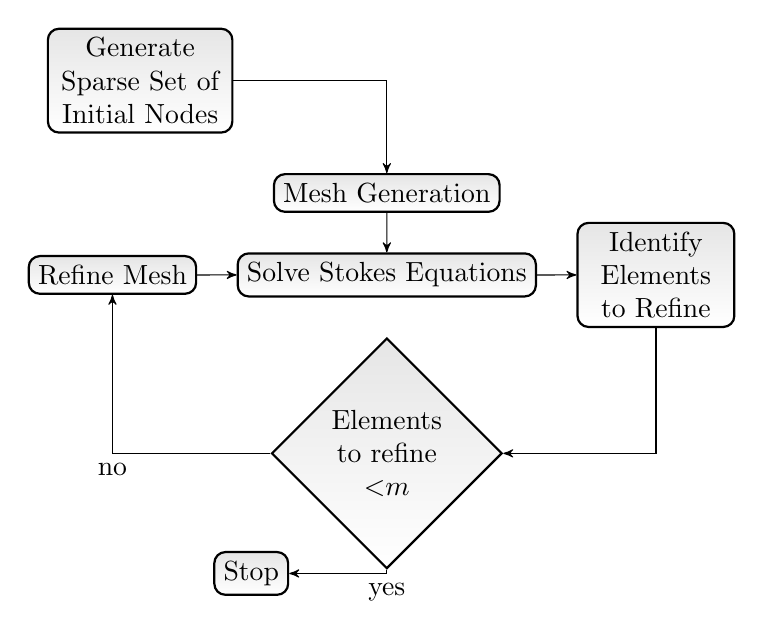
\begin{tikzpicture}[node distance=5mm and 5mm,scale=.8,
	decision/.style={diamond, draw=black, thick, top color=gray!20, bottom color=white,
	text width=5em, text badly centered, 
	inner sep=.5pt}, 
	block/.style ={rectangle, draw=black, thick, top color=gray!20, bottom color=white,
	rounded corners,
},] 

\node (init)[block, text badly centered,text width=6em] {Generate Sparse Set of Initial Nodes};
\pause 
\node(gen) [block,below right=of init] {Mesh Generation};
\draw[-stealth'] (init) -| (gen); 
\pause

\node(solve)[block,below=of gen] {Solve Stokes Equations};   
\draw[-stealth'] (gen) -- (solve);
\pause

\node(elements) [block,right=of solve,text width=5em,text badly centered] {Identify Elements to Refine}; 
\draw[-stealth'] (solve) -- (elements);
\pause

\node(decide)[decision,below=of solve] {Elements to refine $<$$m$};  
\draw[-stealth'] (elements) |- (decide); 
\pause

\node(update) [block,left=of solve] {Refine Mesh}; 
\draw[-stealth'] (decide) -| node [below] {no} (update);
\pause

\draw[-stealth'] (update) -- (solve); 
\pause
 
\node (stop)[block,below left=of decide] {Stop}; 
\draw[-stealth'] (decide) |- node [below] {yes} (stop); 

\end{tikzpicture}\\ 
\only<1-7>{~}
\only<8>{How is this efficient?}
\end{frame}

\begin{frame}{The Error Indicator and Relative Error Measurement}
\begin{itemize}
\item Typically we take some measure of the solution gradient as an indicator of elemental error. 
\pause
\item These measures are called ``a posteriori'' (after the fact) estimates because we must solve the problem before we get an estimate of error. 
\pause
\item For the Stokes equations we have three indicators: $u,v,p$. 
\pause
\end{itemize}
Let $\theta^e$ be the indicator for an element $e$ with vertex nodes $i,j,k$:
\pause
$$E_e=\frac{(\mbox{Maximum nodal value} - \mbox{Minimum Nodal Value})_e}{\mbox{Average difference in max and min nodal values over all elements}}$$
$$E_e = \frac{\max\left(\theta^e_i,\theta^e_j,\theta^e_k\right)-\min\left(\theta^e_i,\theta^e_j,\theta^e_k\right)}{\frac{1}{nele}\sum^{nele}_{n=1}\left[\max\left(\theta^n_i,\theta^n_j,\theta^n_k\right)-\min\left(\theta^n_i,\theta^n_j,\theta^n_k\right)\right]}\label{eqn:err}$$
\end{frame}
%%%%%%%%%%%%%%%%%%%%%%%%%%%%%%%%%%%%%%

%%%%%%%%%%%%%%%%%%%%%%%%%%%%%%%%%%%%%
\section{Model Results}
\subsection{0}
\begin{frame}{Simulation Model Results - Verification}
\pause
\begin{figure}
\subfigure[Velocity Field]{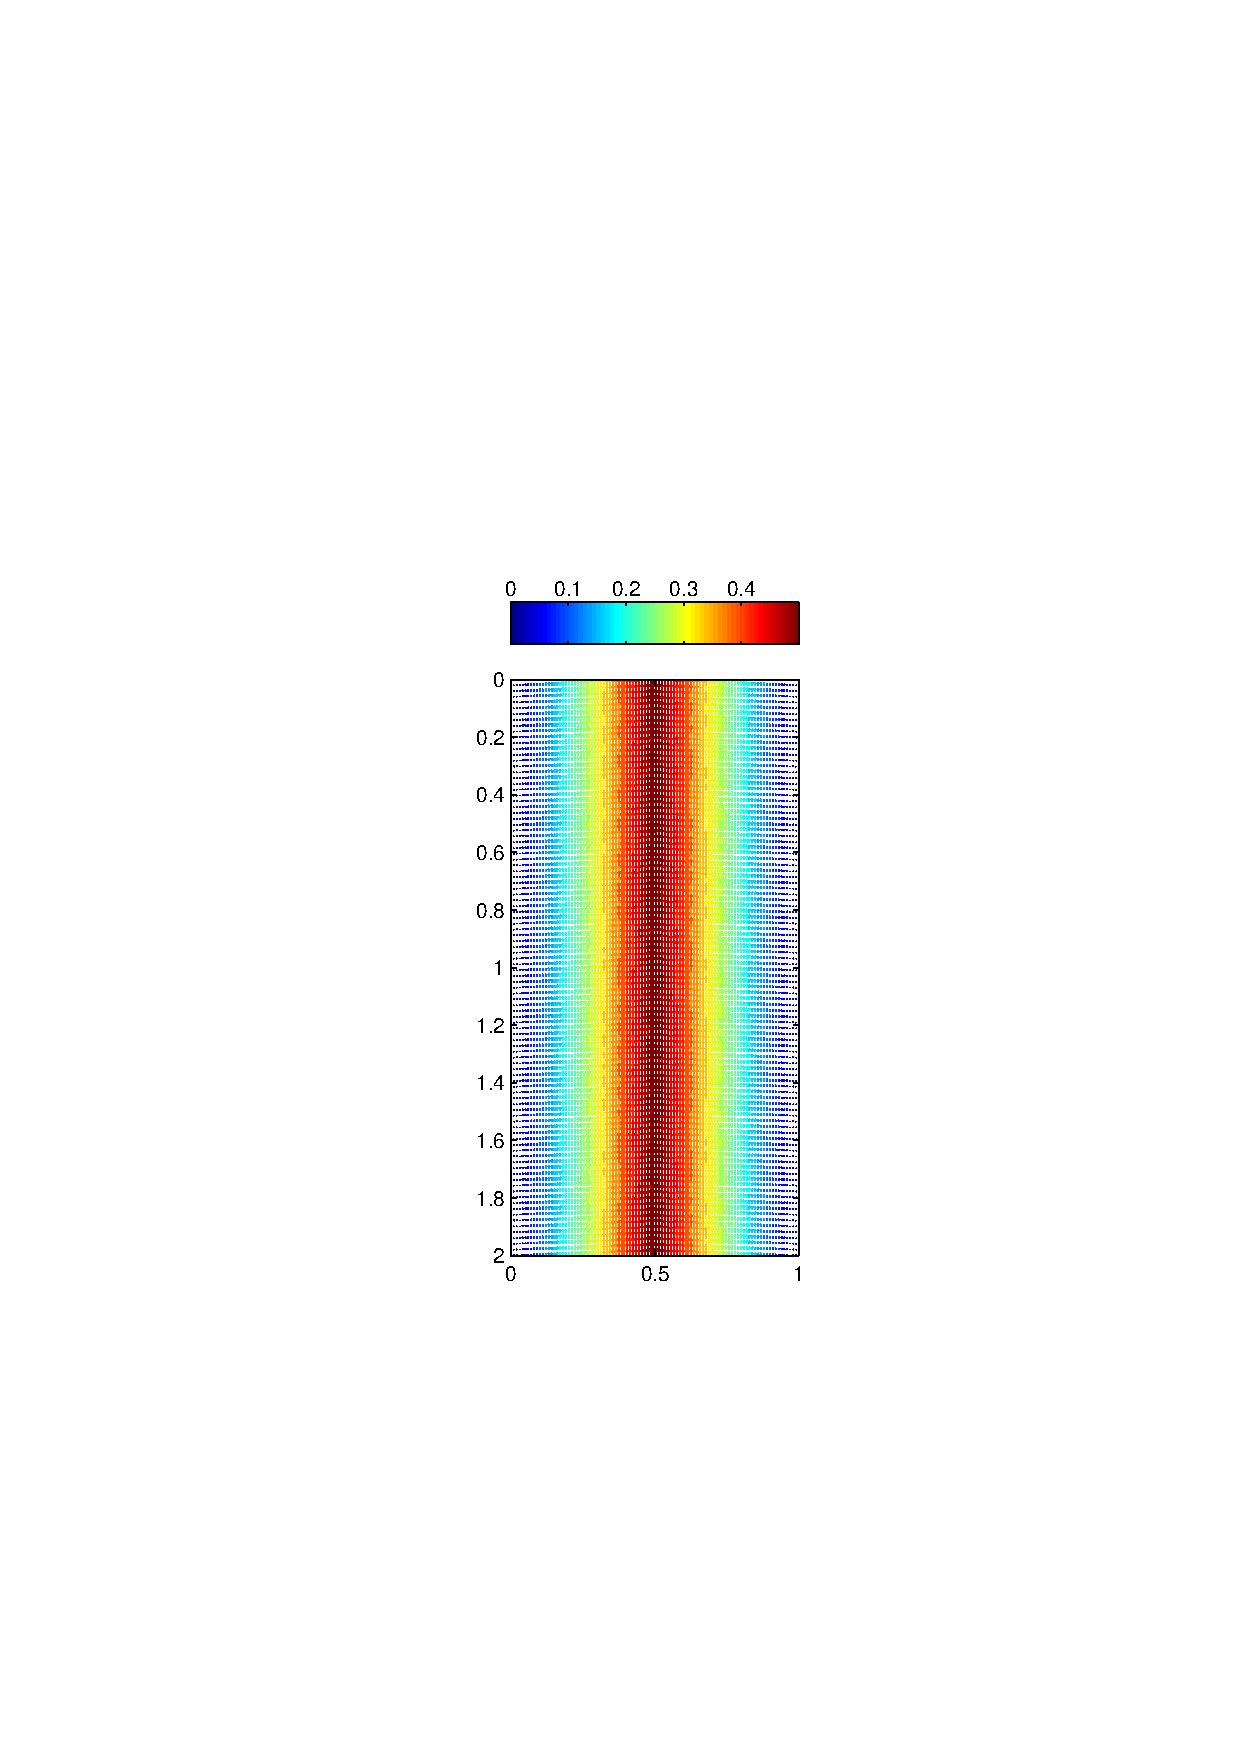
\includegraphics[width=.25\textwidth]{../plots/stokes_vectors_0.pdf}}
\subfigure[Velocity Contours]{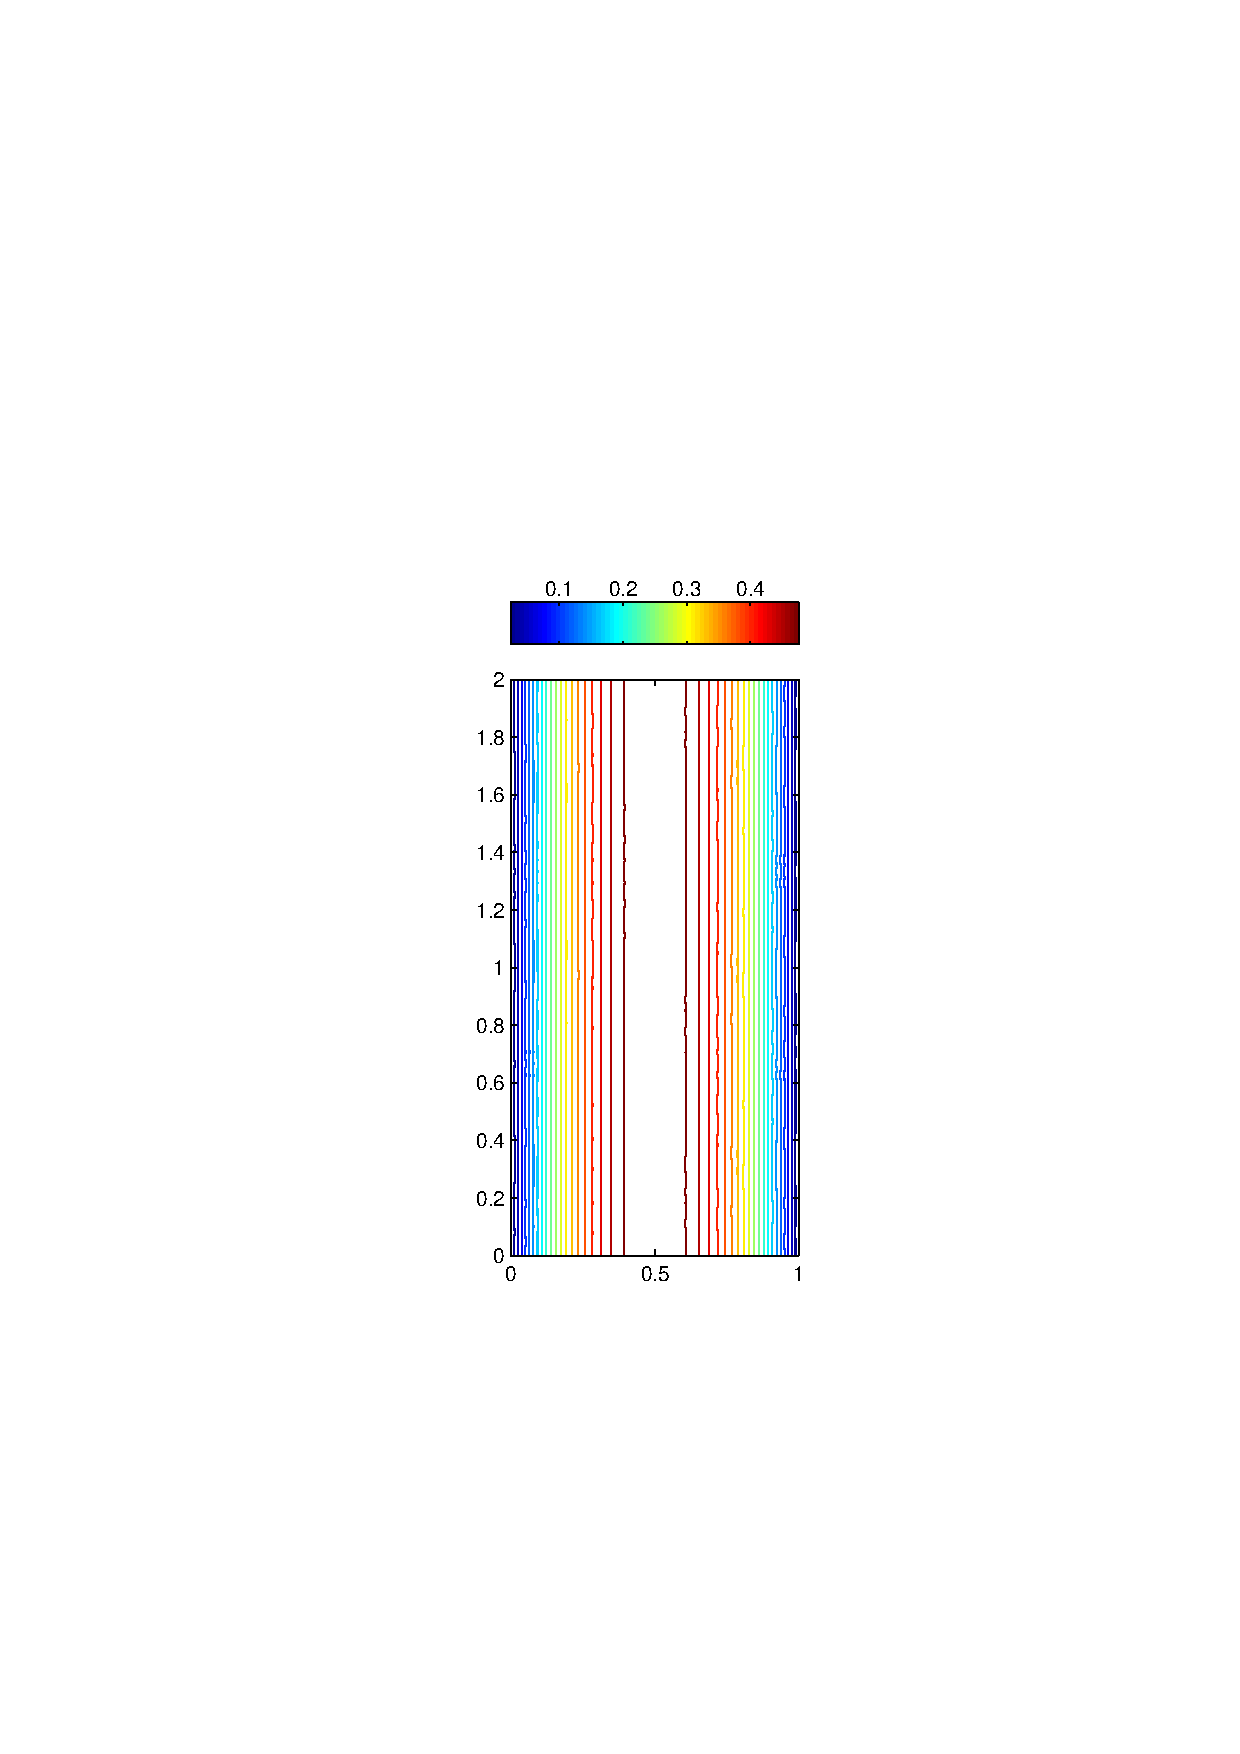
\includegraphics[width=.25\textwidth]{../plots/stokes_velocity_0.pdf}}
\subfigure[Streamlines and Pressure Contours]{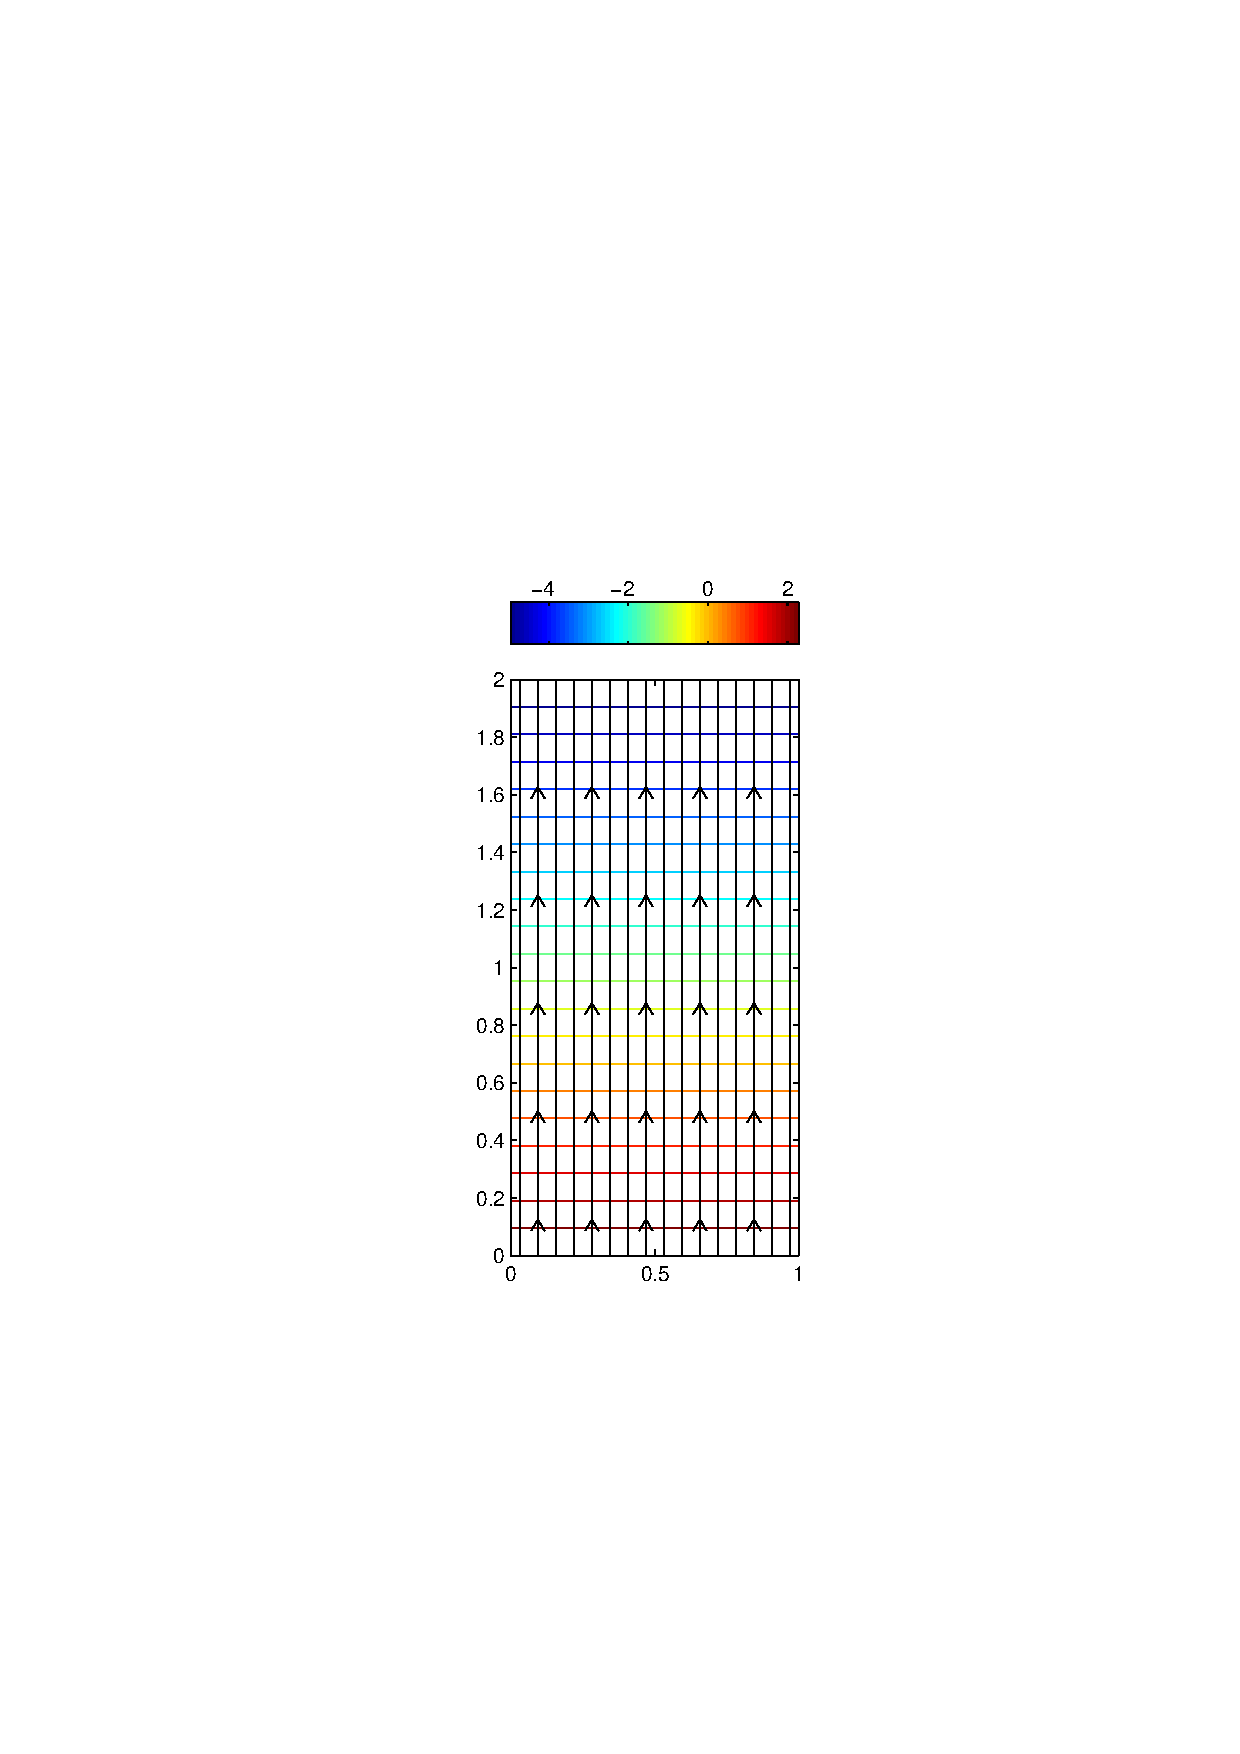
\includegraphics[width=.255\textwidth]{../plots/stokes_solution_0.pdf}}
\end{figure}
\end{frame}
\setcounter{subfigure}{0}
%%%%%%%%%%%%%%%%%%%%%%%%%%%%%%%%%%%%%%

%%%%%%%%%%%%%%%%%%%%%%%%%%%%%%%%%%%%%
\subsection{1}
\begin{frame}{1 Obstruction}
\begin{figure}
\subfigure[Velocity Field]{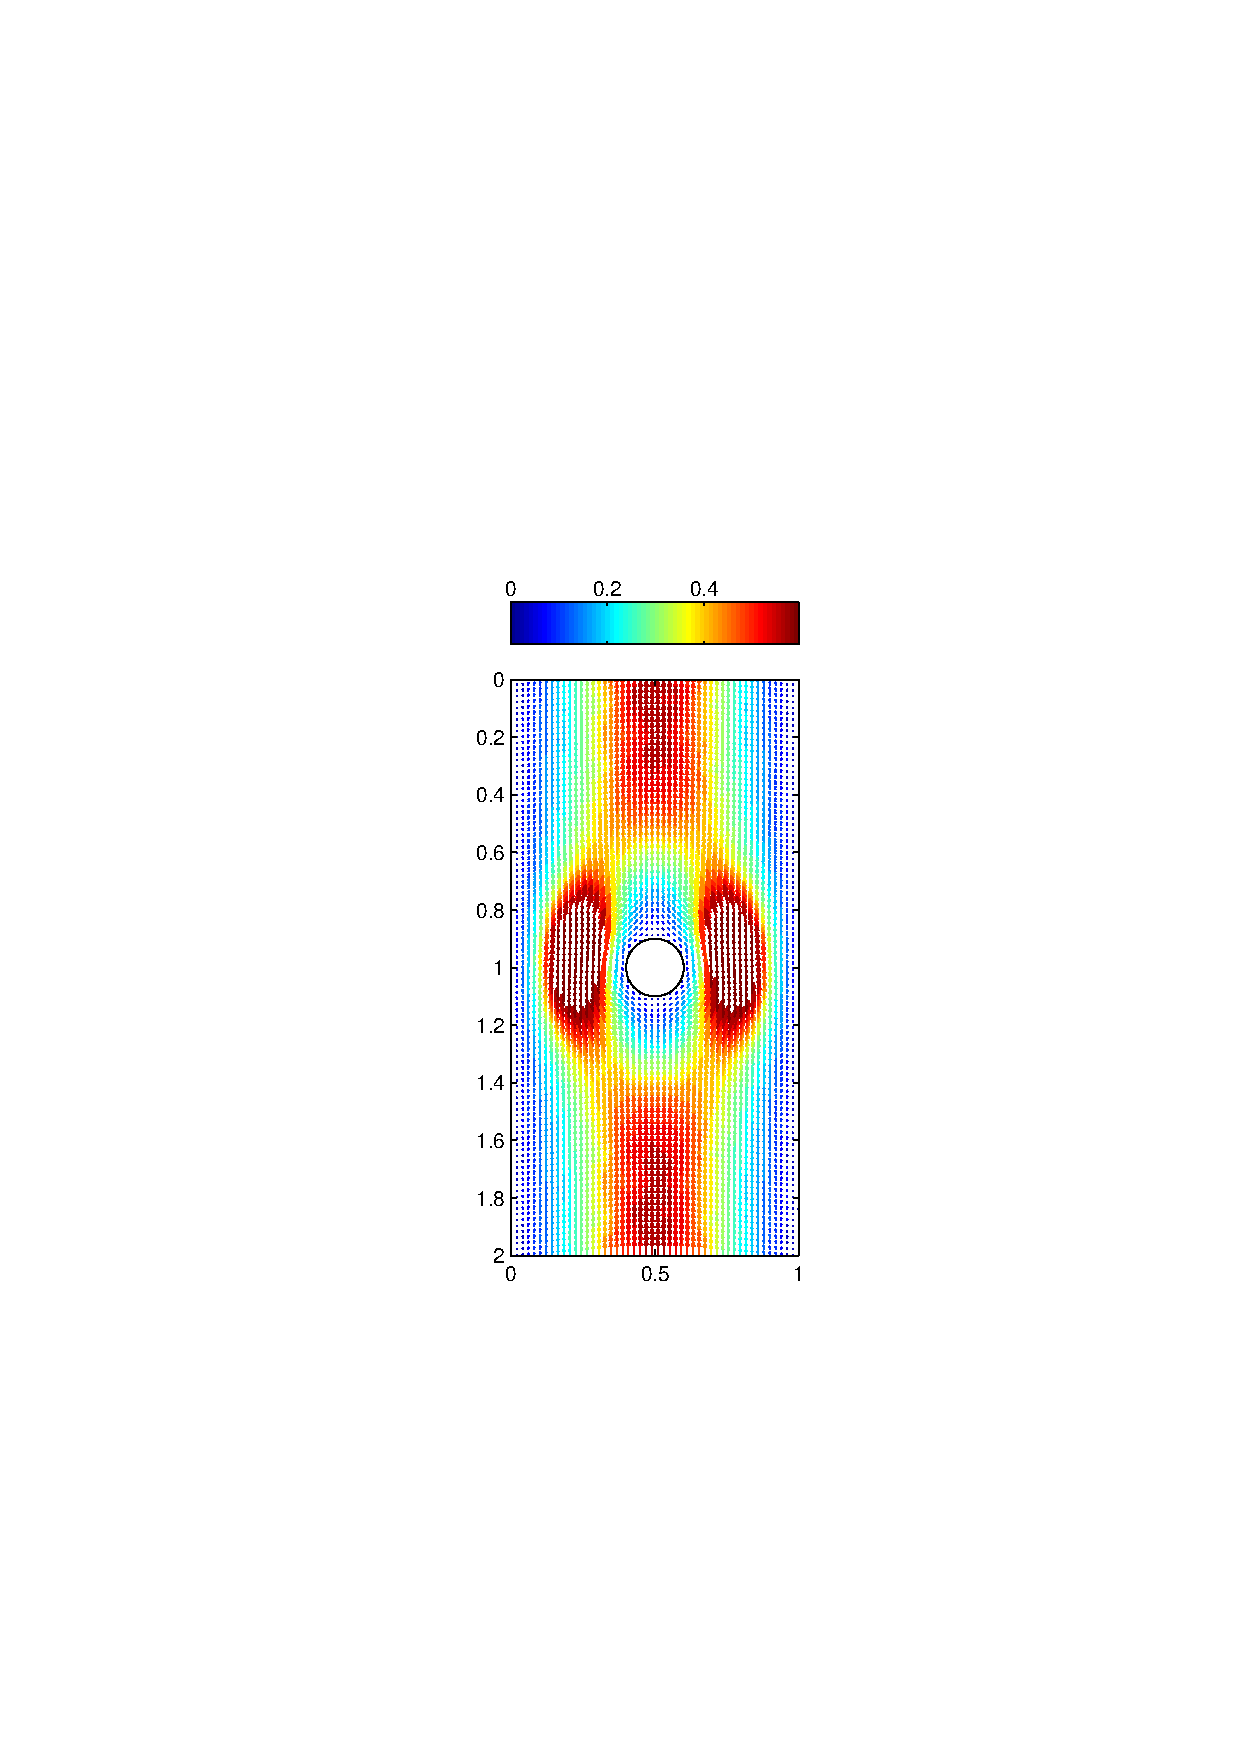
\includegraphics[width=.25\textwidth]{../plots/stokes_vectors_1.pdf}}
\subfigure[Velocity Contours]{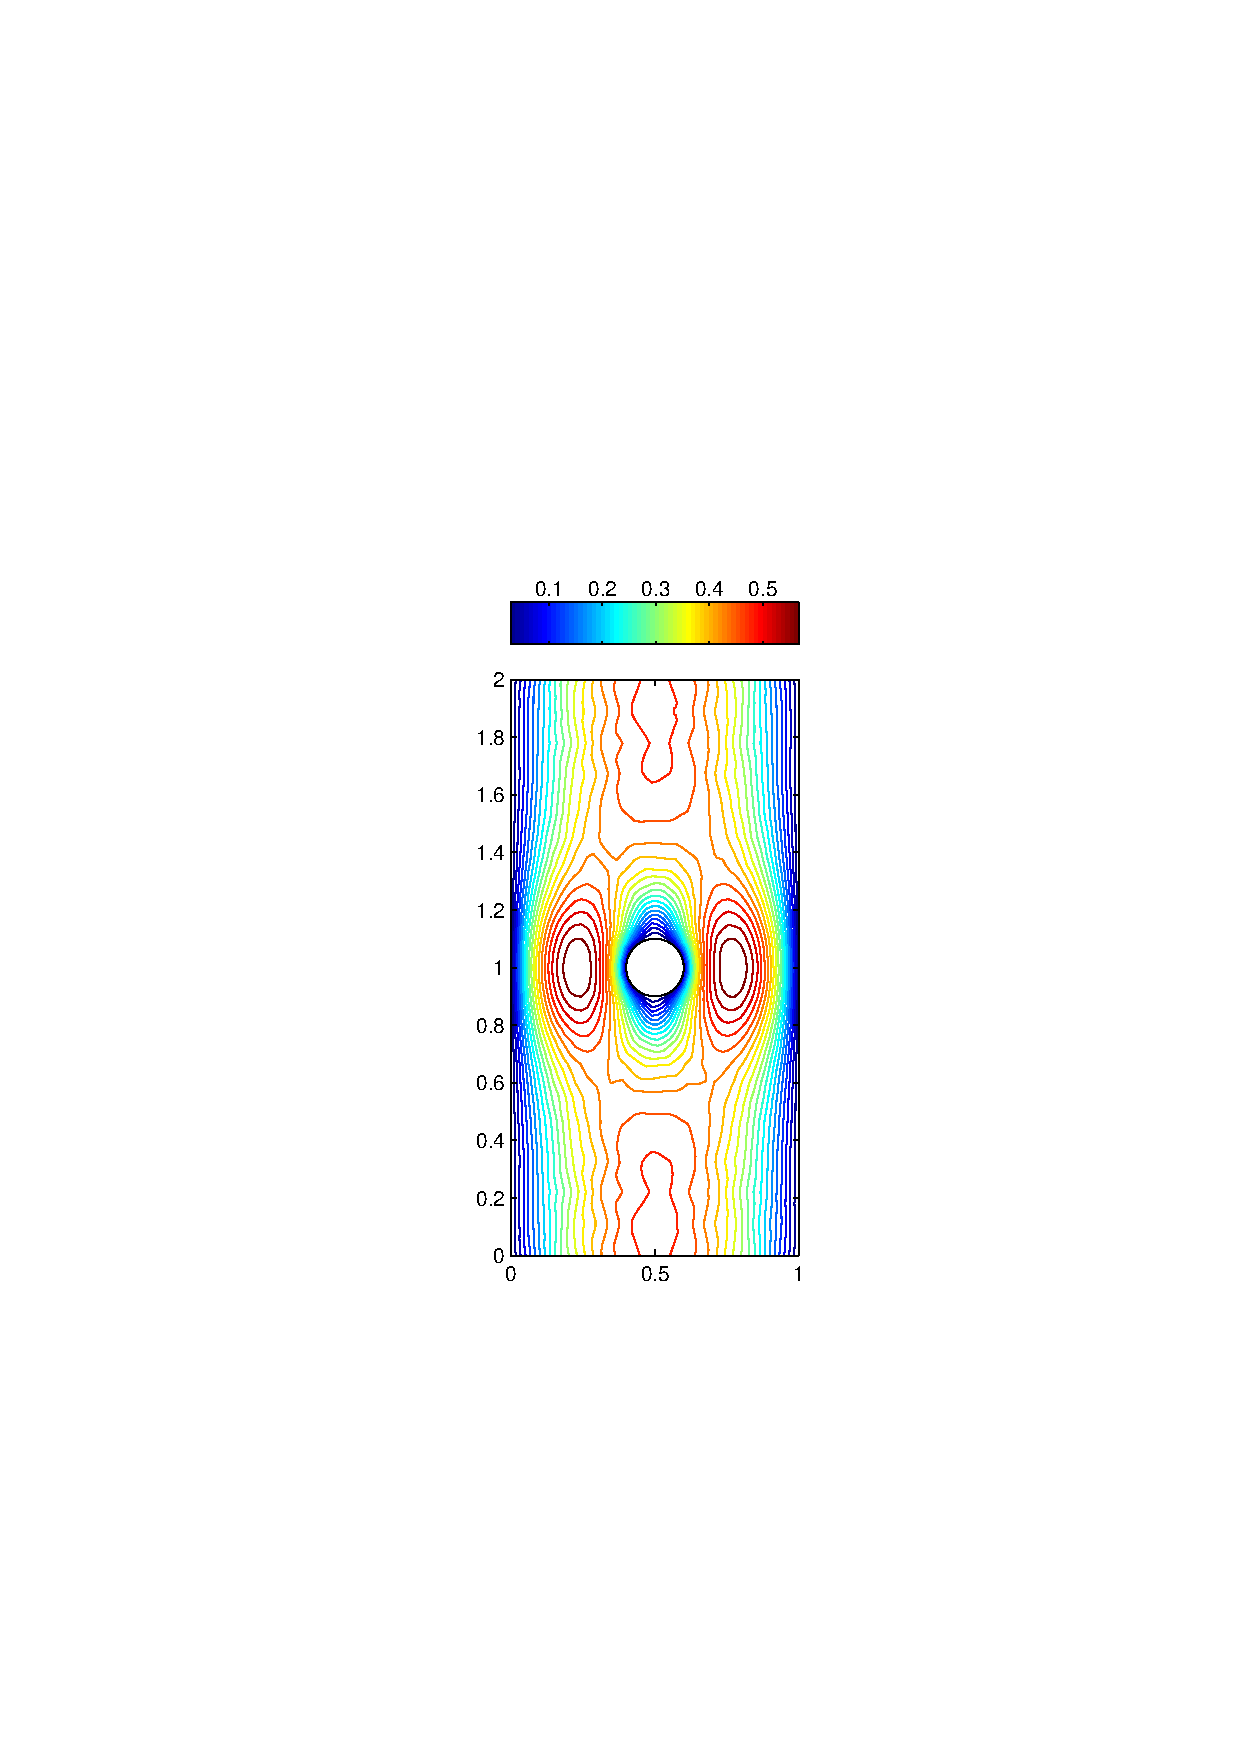
\includegraphics[width=.25\textwidth]{../plots/stokes_velocity_1.pdf}}
\subfigure[Streamlines and Pressure Contours]{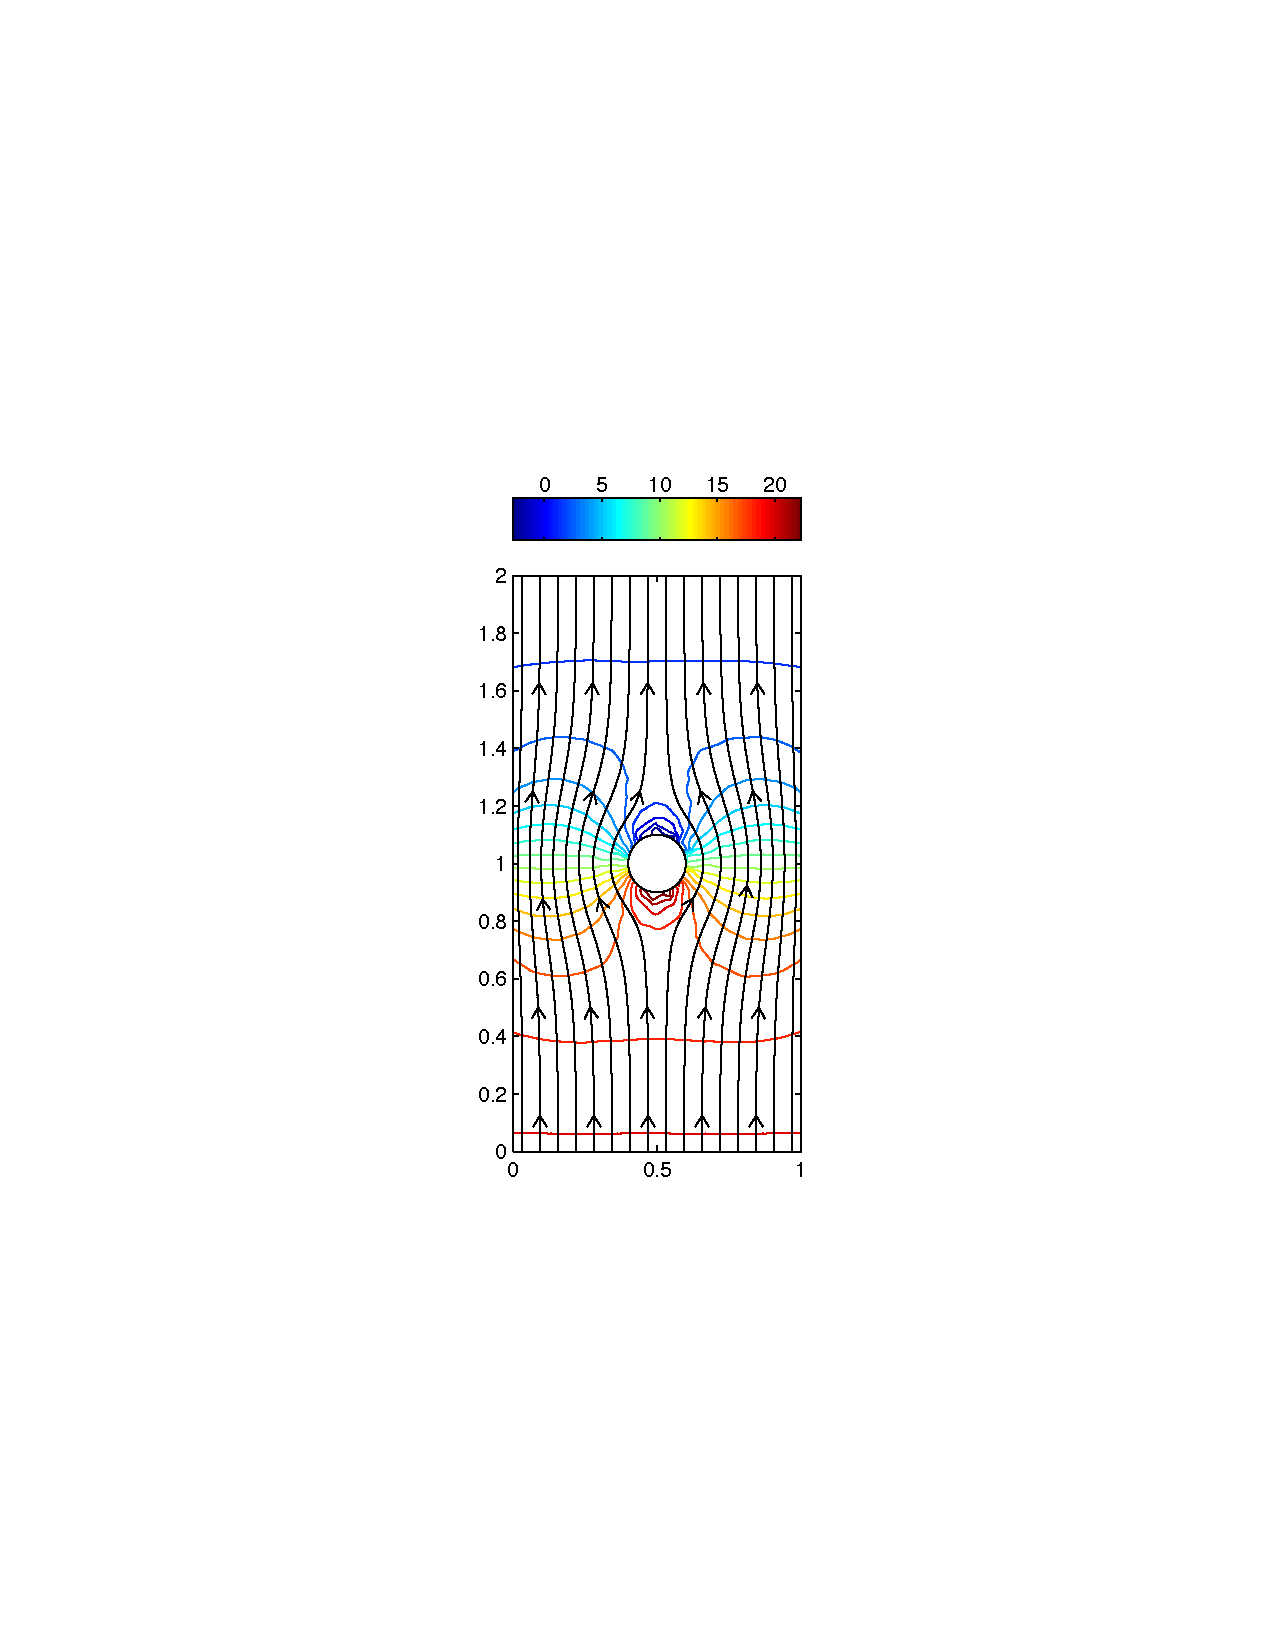
\includegraphics[width=.25\textwidth]{../plots/stokes_solution.pdf}}
\end{figure}
\end{frame}
\setcounter{subfigure}{0}
%%%%%%%%%%%%%%%%%%%%%%%%%%%%%%%%%%%%%%

%%%%%%%%%%%%%%%%%%%%%%%%%%%%%%%%%%%%%
\subsection{5}
\begin{frame}{5 Obstructions}
\begin{figure}
\subfigure[Velocity Field]{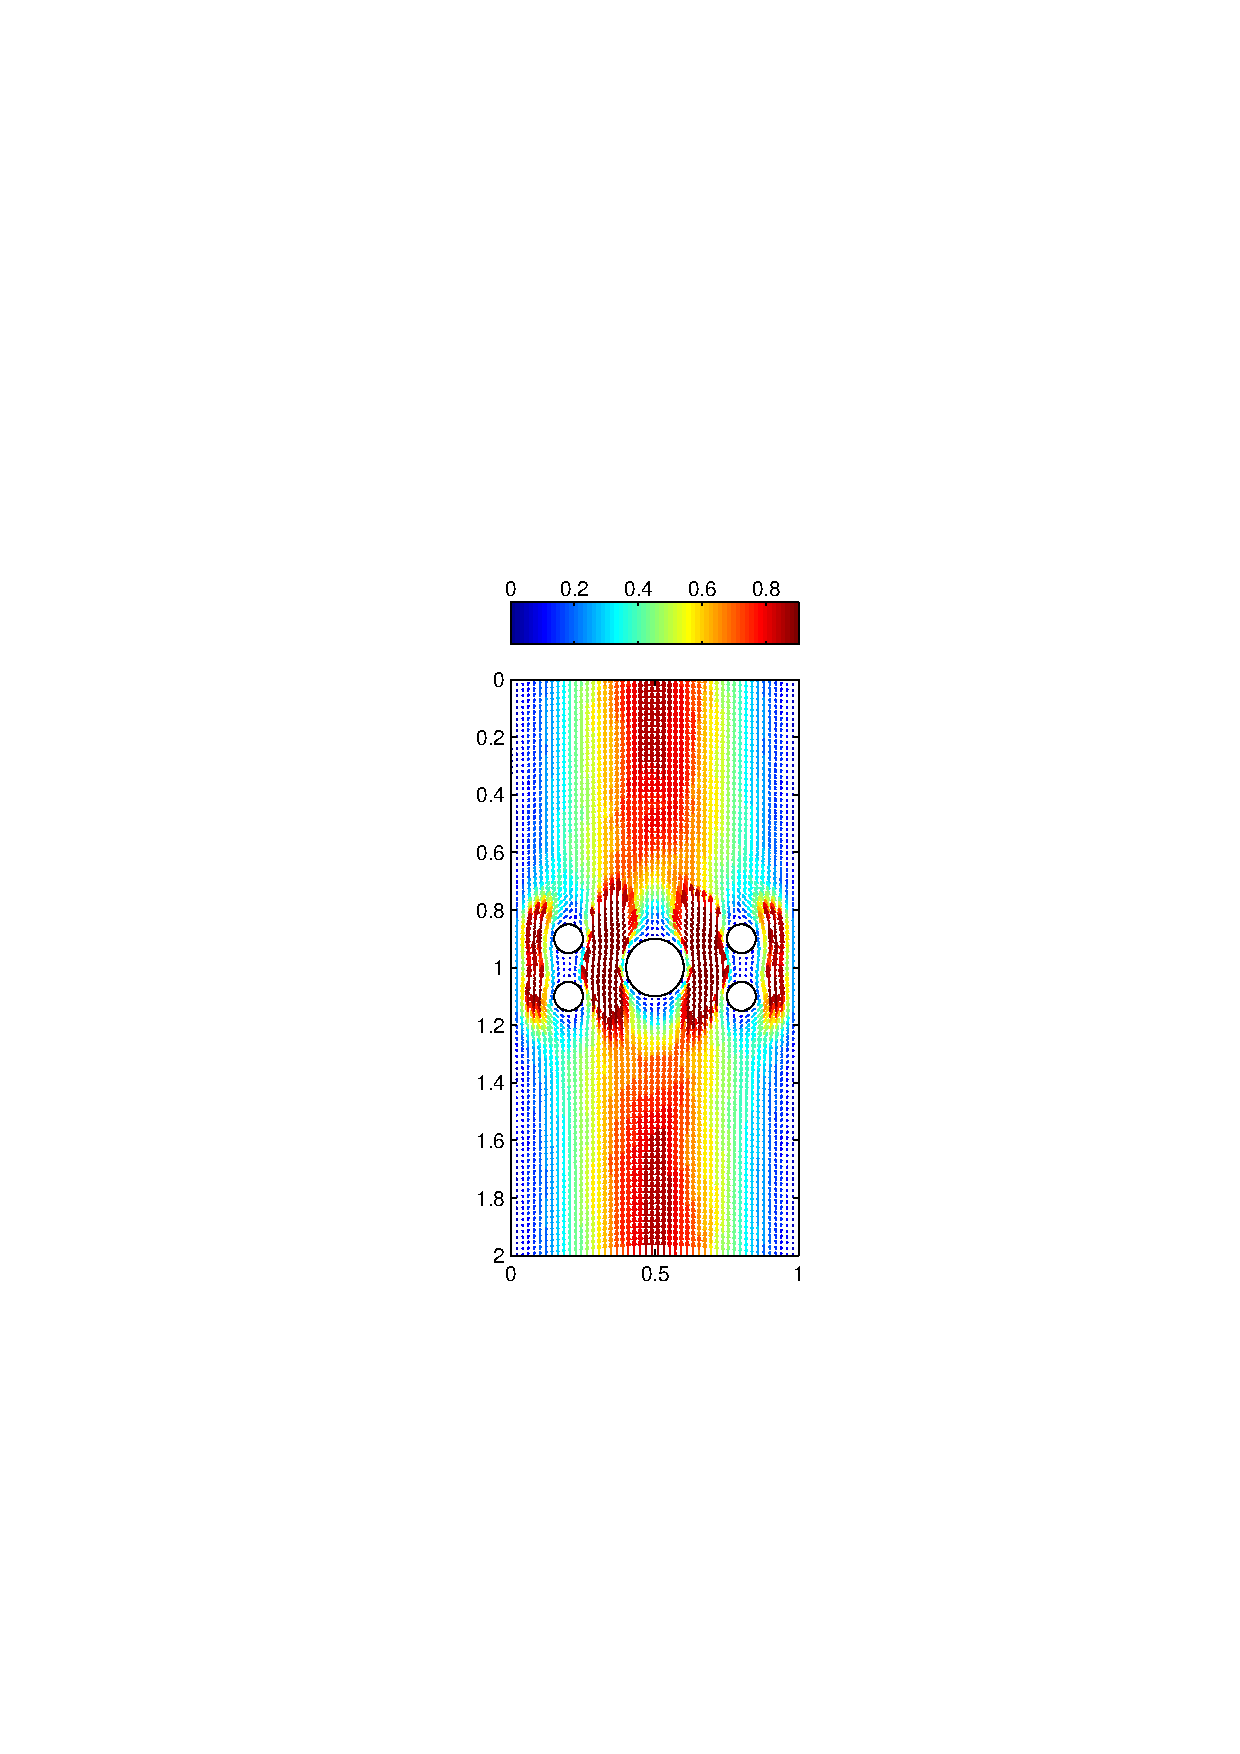
\includegraphics[width=.25\textwidth]{../plots/stokes_vectors_5.pdf}}
\subfigure[Velocity Contours]{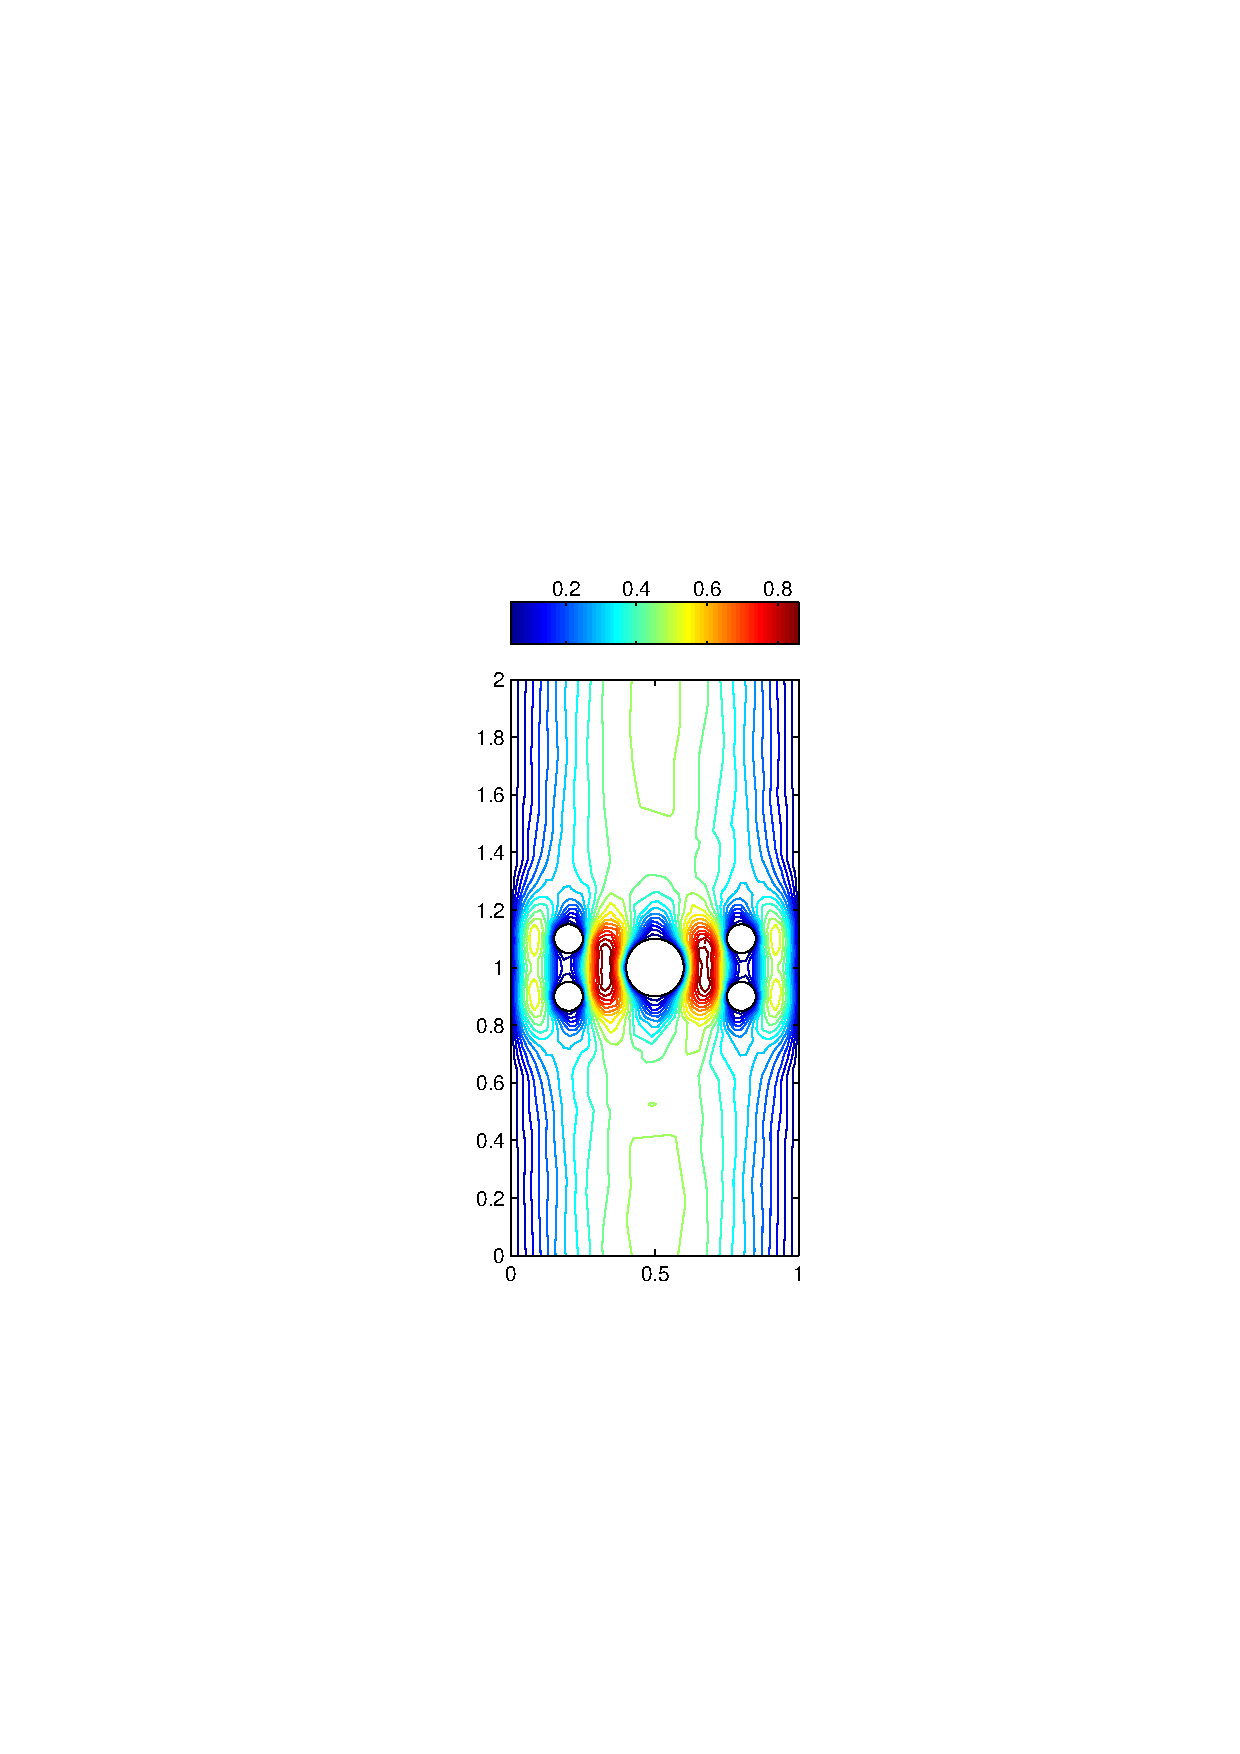
\includegraphics[width=.25\textwidth]{../plots/stokes_velocity_5.pdf}}
\subfigure[Streamlines and Pressure Contours]{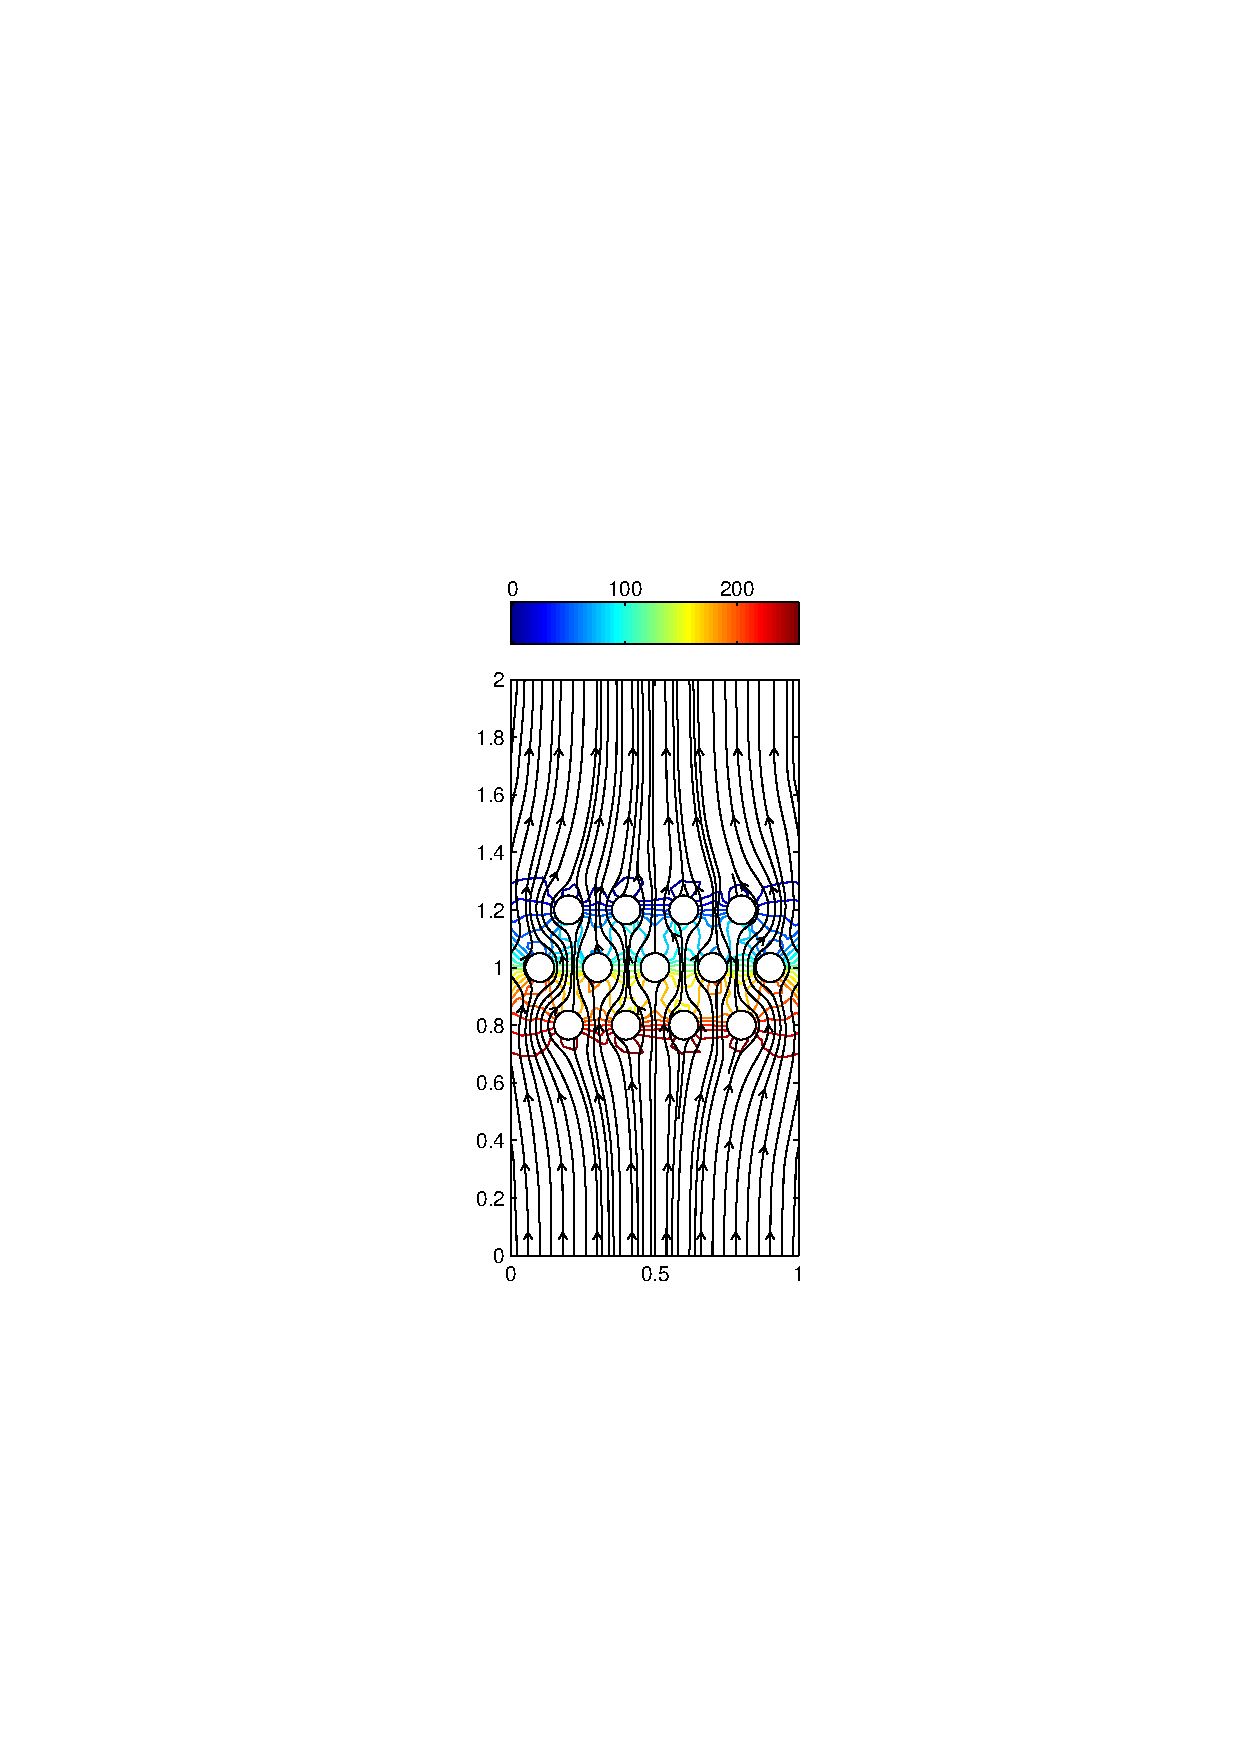
\includegraphics[width=.25\textwidth]{../plots/stokes_solution_5.pdf}}
\end{figure}
\end{frame}
\setcounter{subfigure}{0}
%%%%%%%%%%%%%%%%%%%%%%%%%%%%%%%%%%%%%%

%%%%%%%%%%%%%%%%%%%%%%%%%%%%%%%%%%%%%
\subsection{13}
\begin{frame}{13 obstructions}
\begin{figure}
\subfigure[Velocity Field]{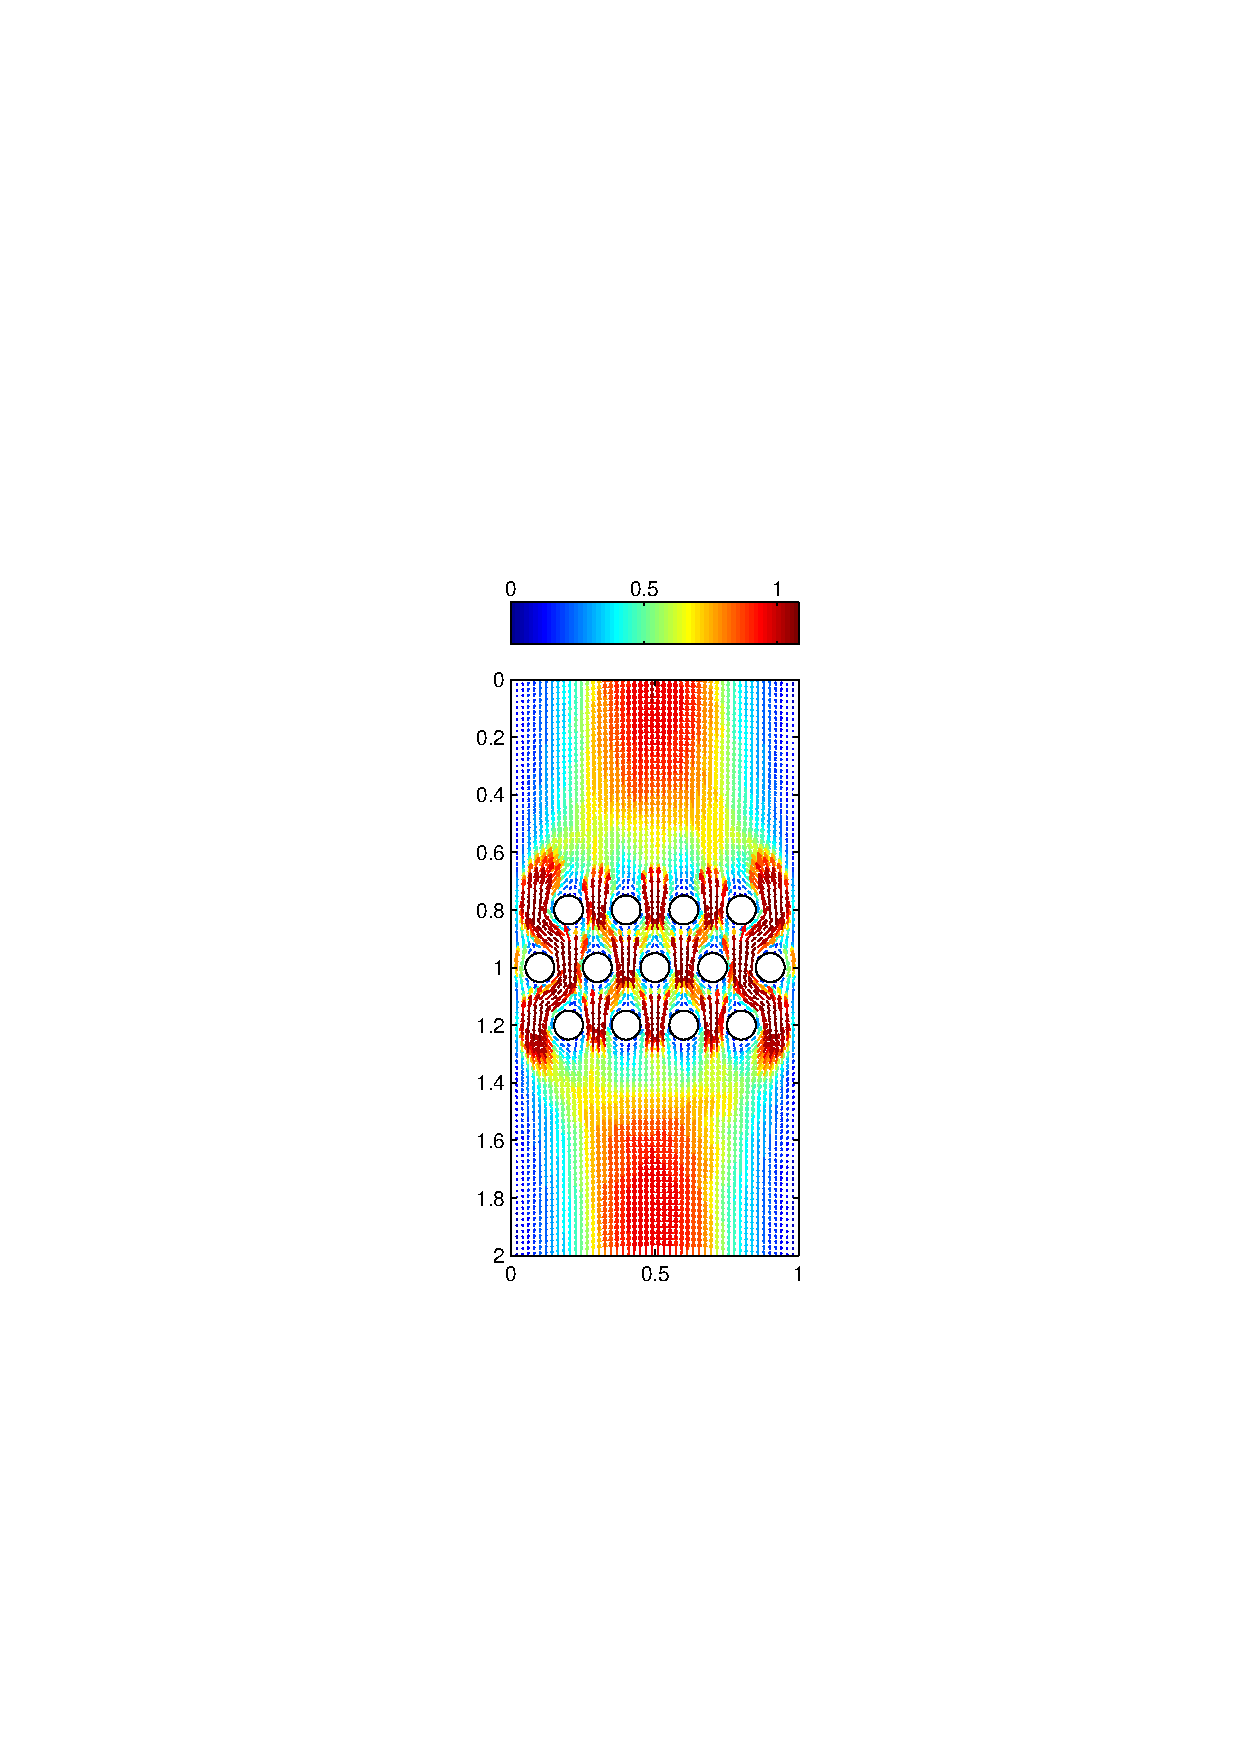
\includegraphics[width=.25\textwidth]{../plots/stokes_vectors_13.pdf}}
\subfigure[Velocity Contours]{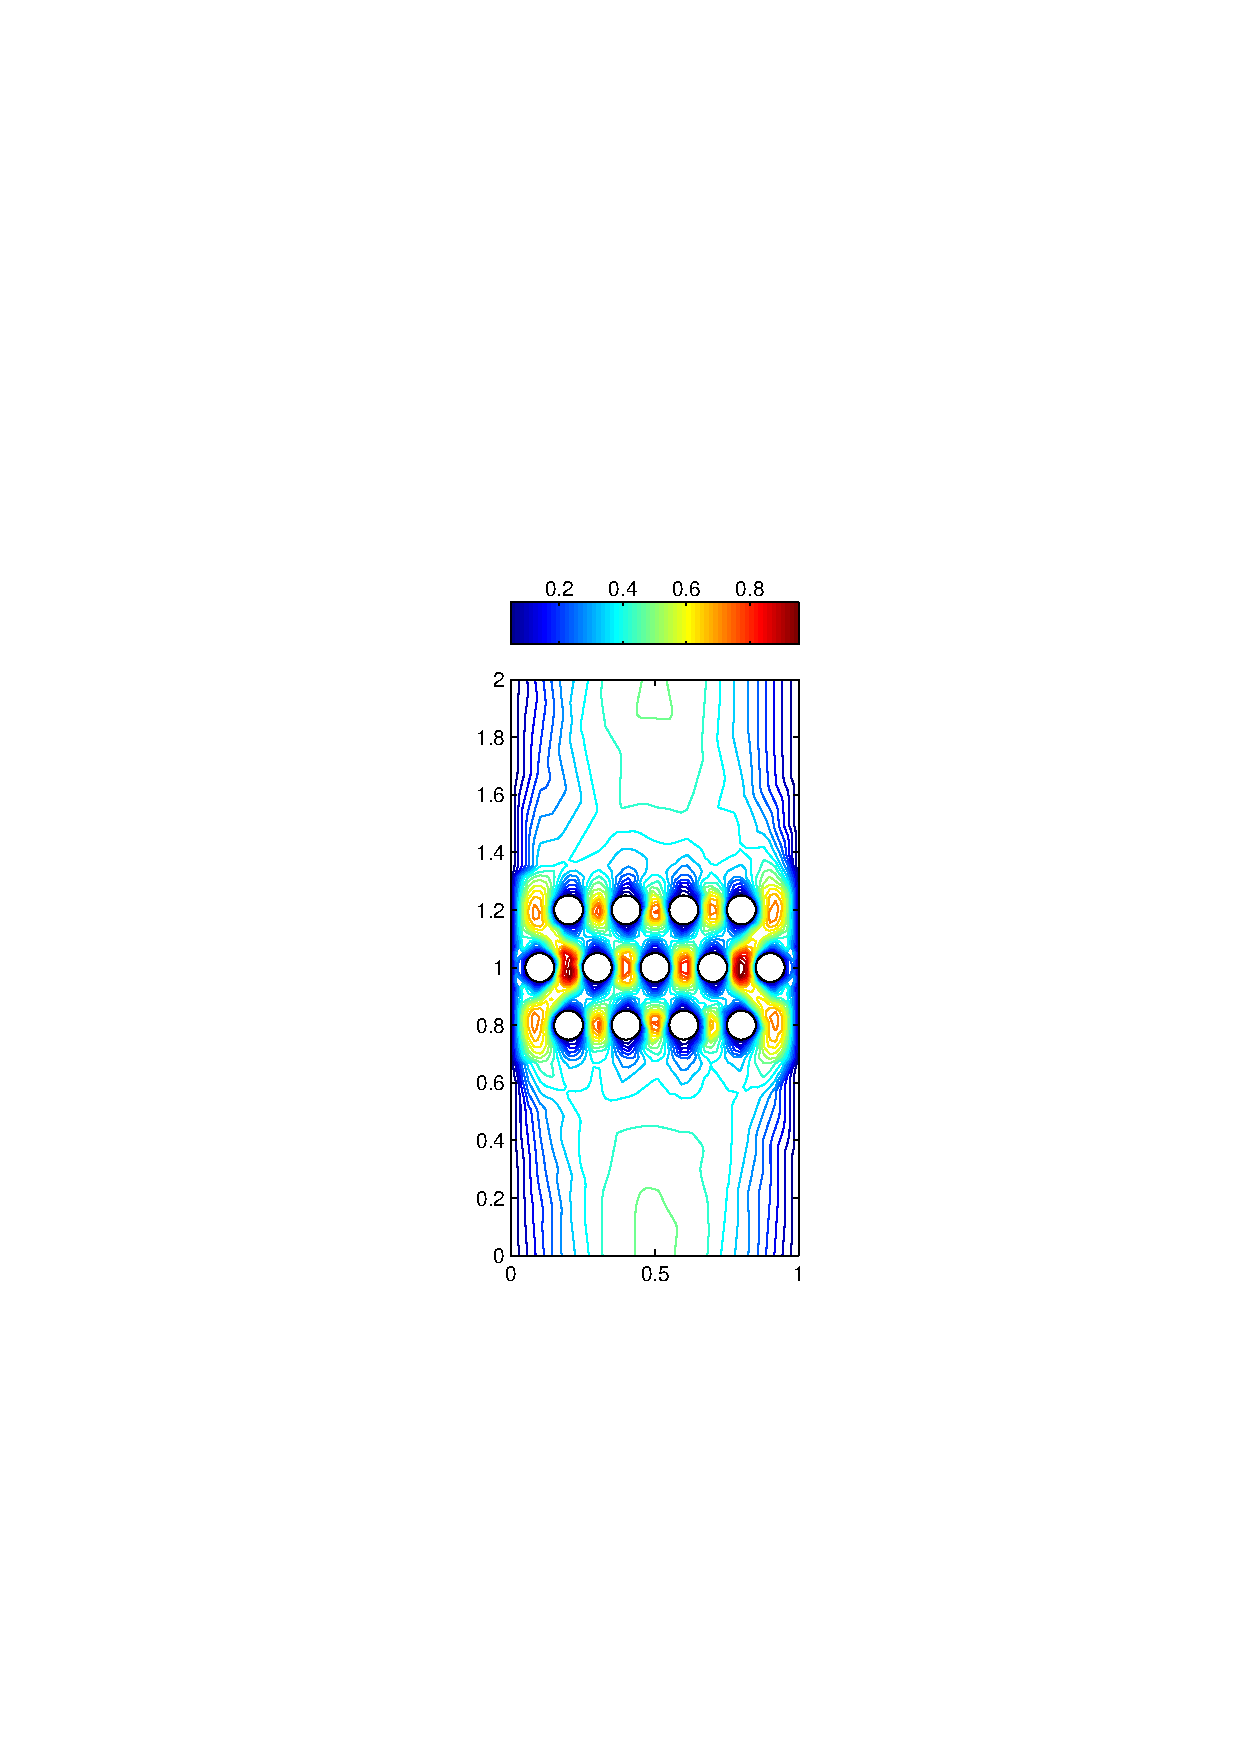
\includegraphics[width=.25\textwidth]{../plots/stokes_velocity_13.pdf}}
\subfigure[Streamlines and Pressure Contours]{\includegraphics[width=.25\textwidth]{../plots/stokes_solution_13.pdf}}
\end{figure}
\end{frame}

%%%%%%%%%%%%%%%%%%%%%%%%%%%%%%%%%%%%%%
\subsection{ver2}
\begin{frame}{Additional Verification}
\begin{figure}
\includegraphics[width=.3\textwidth]{cylinders.pdf}
\end{figure}
{\tiny[TQ Education and Training Ltd.]}
\end{frame}
%%%%%%%%%%%%%%%%%%%%%%%%%%%%%%%%%%%%%

%%%%%%%%%%%%%%%%%%%%%%%%%%%%%%%%%%%%%
\section{Meshing Results}
\subsection{show}
\begin{frame}{Meshing Results}
{\hspace{1cm} Pressure \hspace{1cm} Horizontal velocity \hspace{1cm} Vertical velocity}
\only<1>{
	Initial Mesh\\~\\
	\includegraphics[height=.4\textwidth]{../plots/mesh1ele_p.pdf}\hspace{1cm}
	\includegraphics[height=.4\textwidth]{../plots/mesh1ele_p.pdf}\hspace{1cm}
	\includegraphics[height=.4\textwidth]{../plots/mesh1ele_p.pdf}\\~
}
\only<2>{
	Refinement 1\\~\\
	\includegraphics[height=.4\textwidth]{../plots/mesh2ele_p.pdf}\hspace{1cm}
	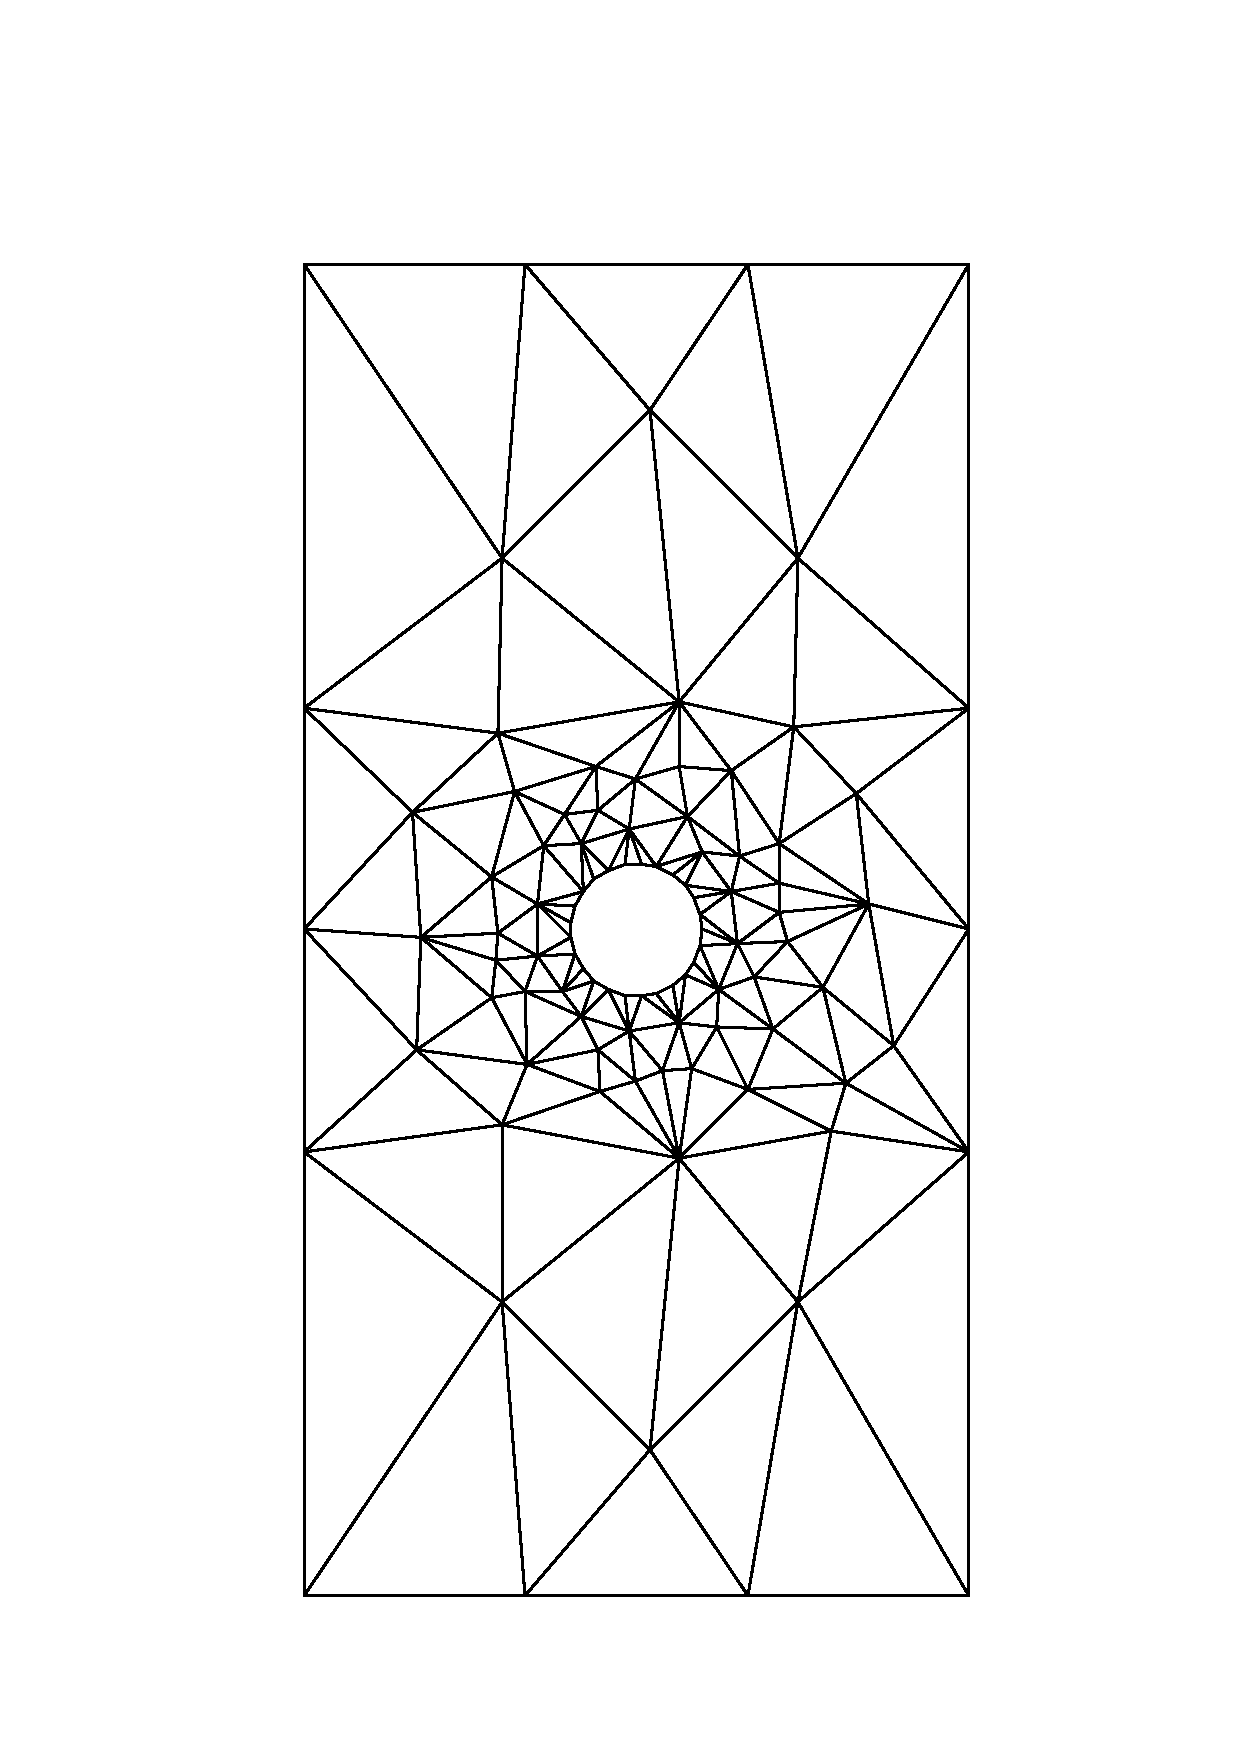
\includegraphics[height=.4\textwidth]{../plots/mesh2ele_u.pdf}\hspace{1cm}
	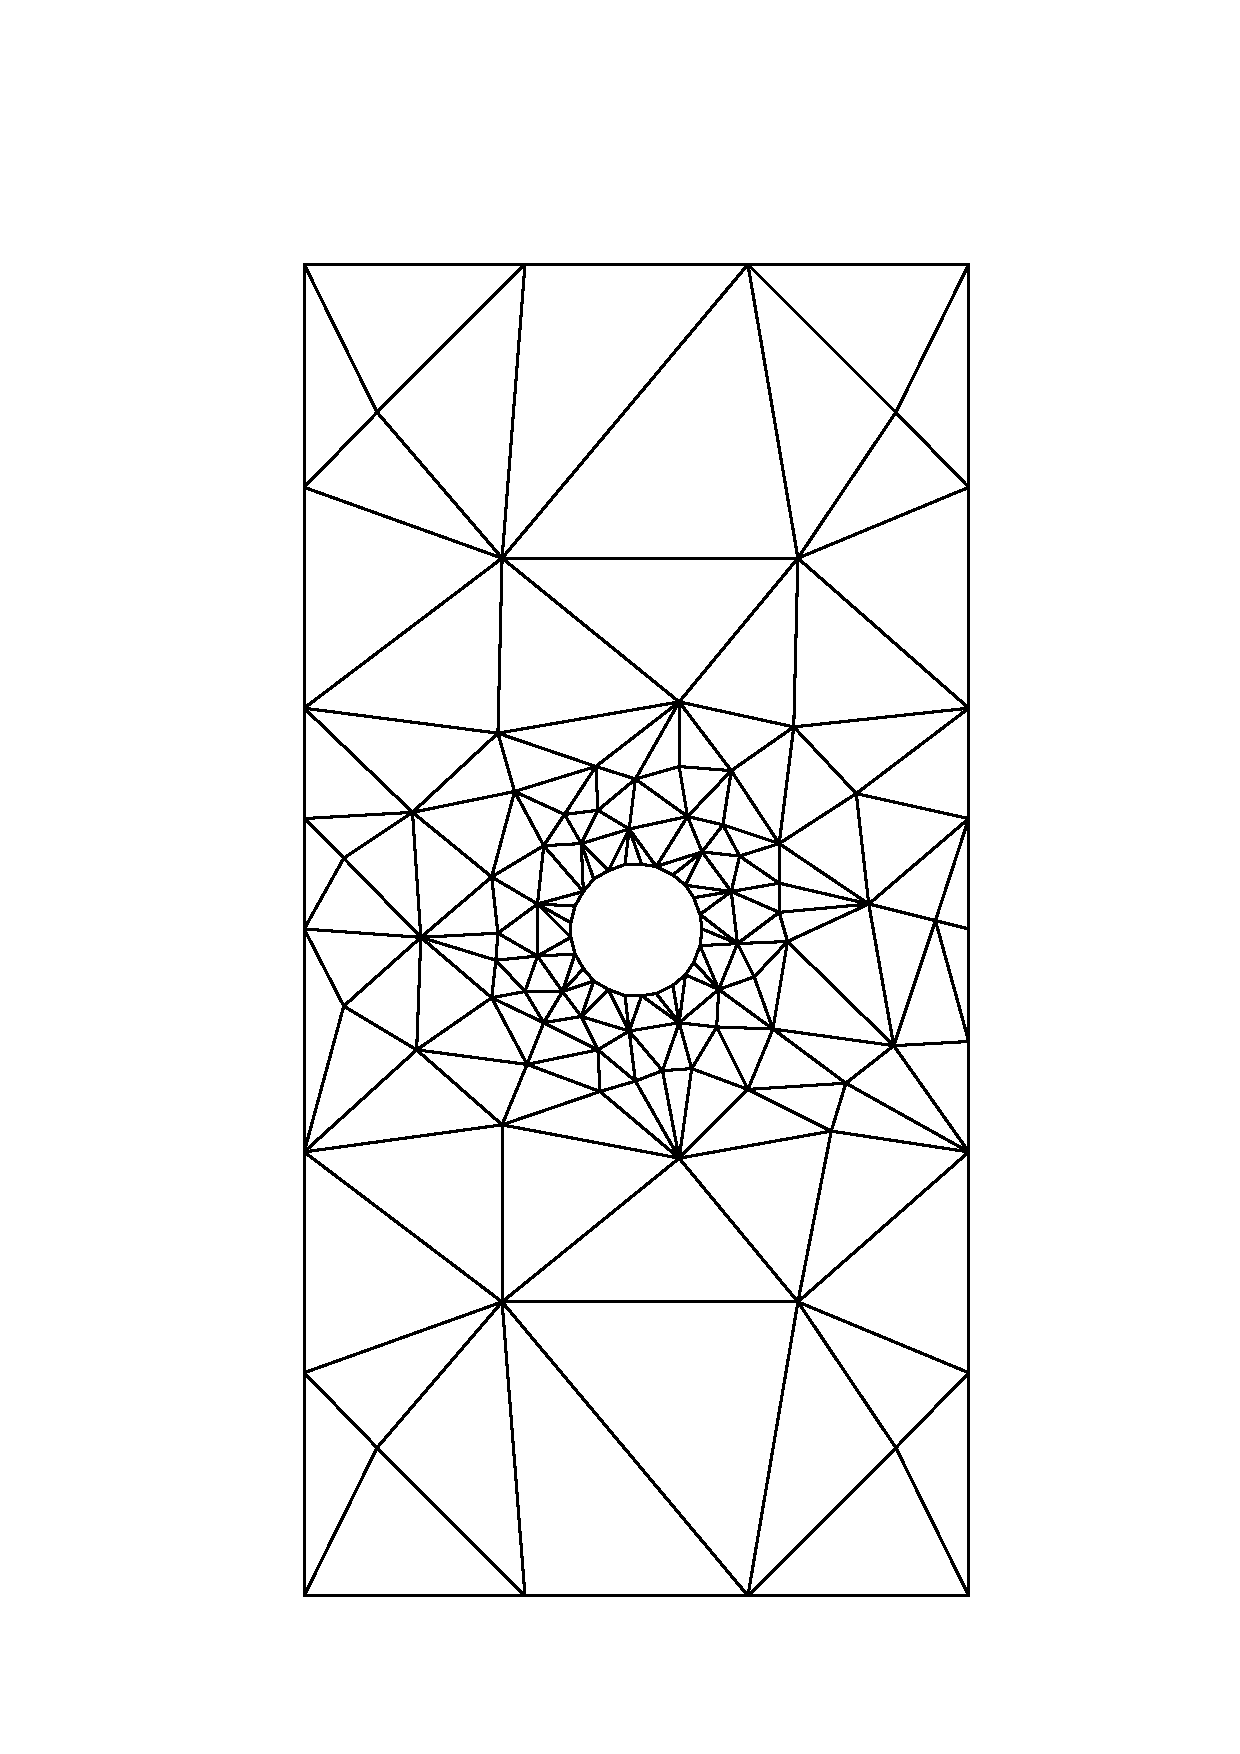
\includegraphics[height=.4\textwidth]{../plots/mesh2ele_v.pdf}\\~
}
\only<3>{
    Refinement 2\\~\\
	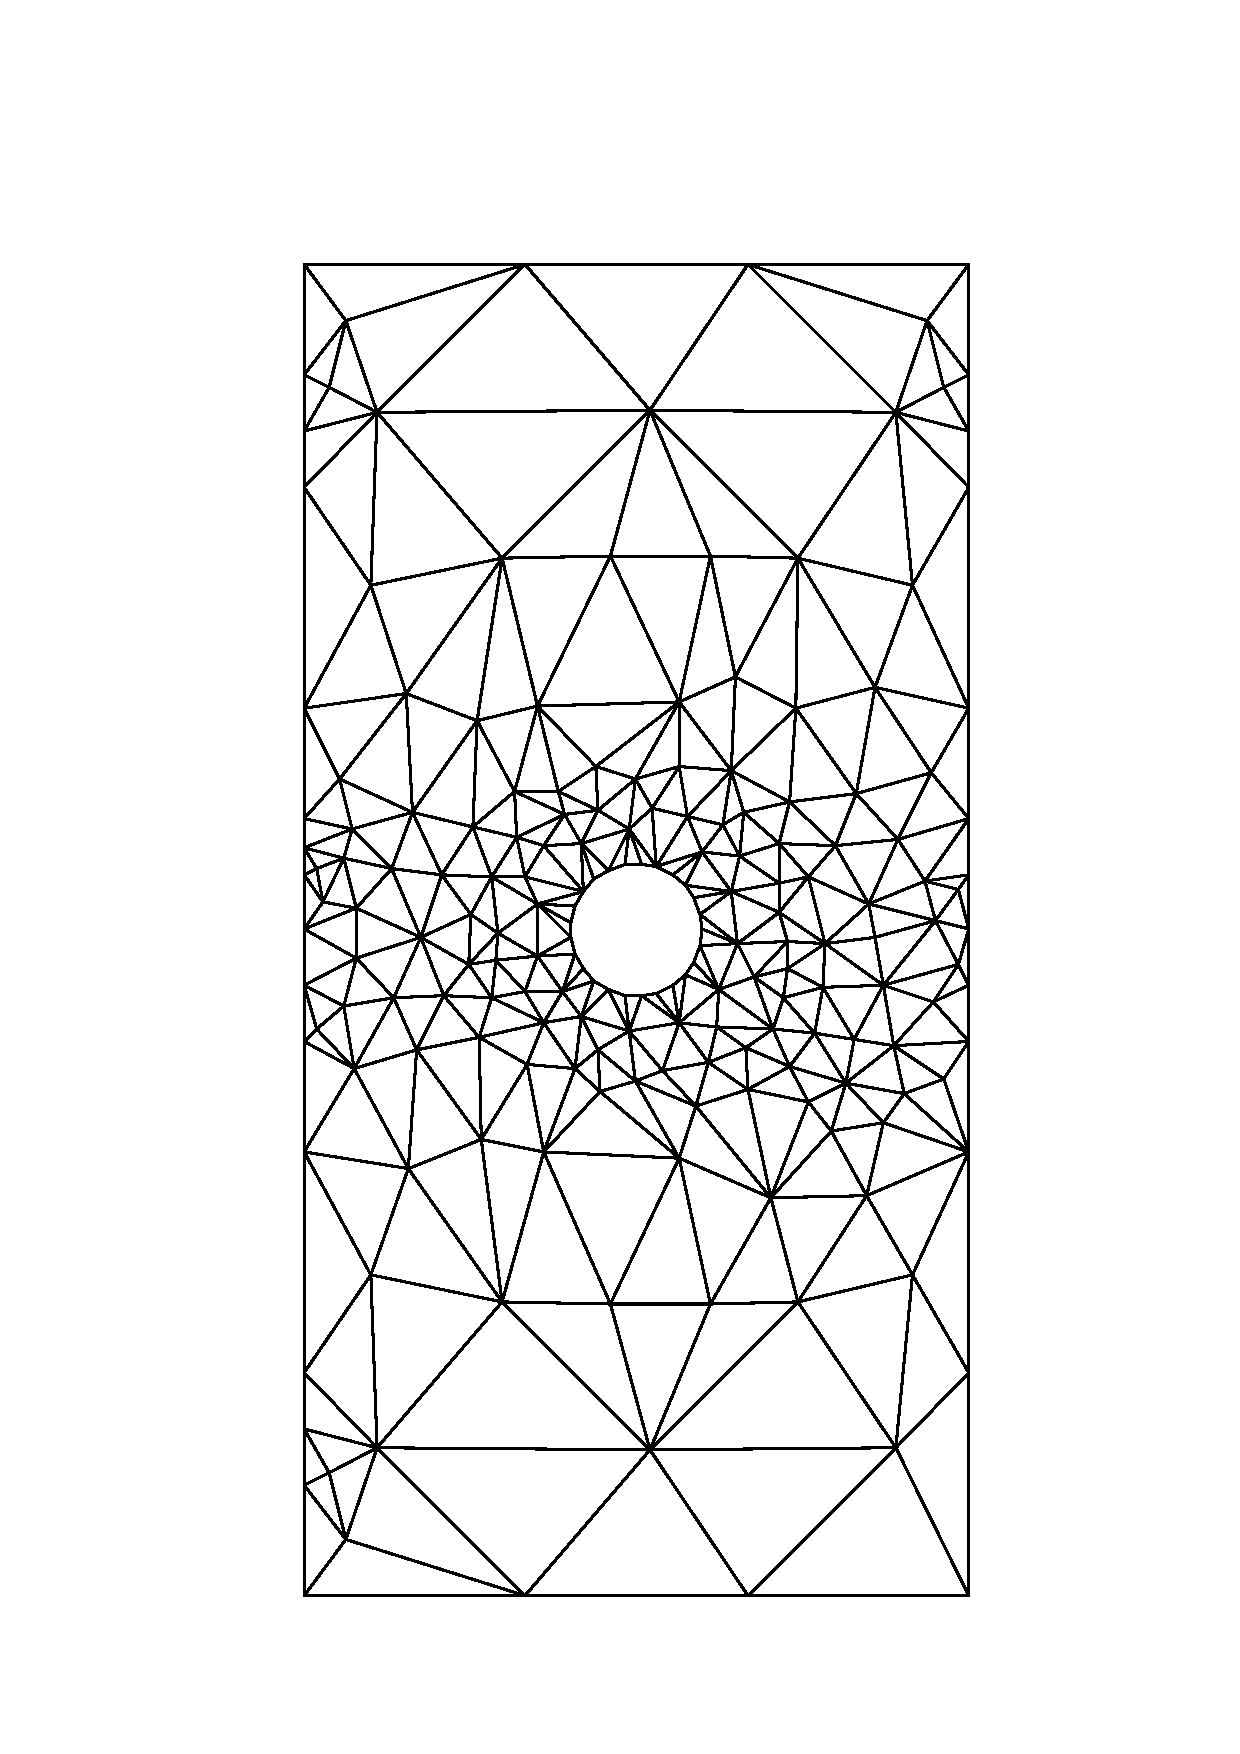
\includegraphics[height=.4\textwidth]{../plots/mesh3ele_p.pdf}\hspace{1cm}
	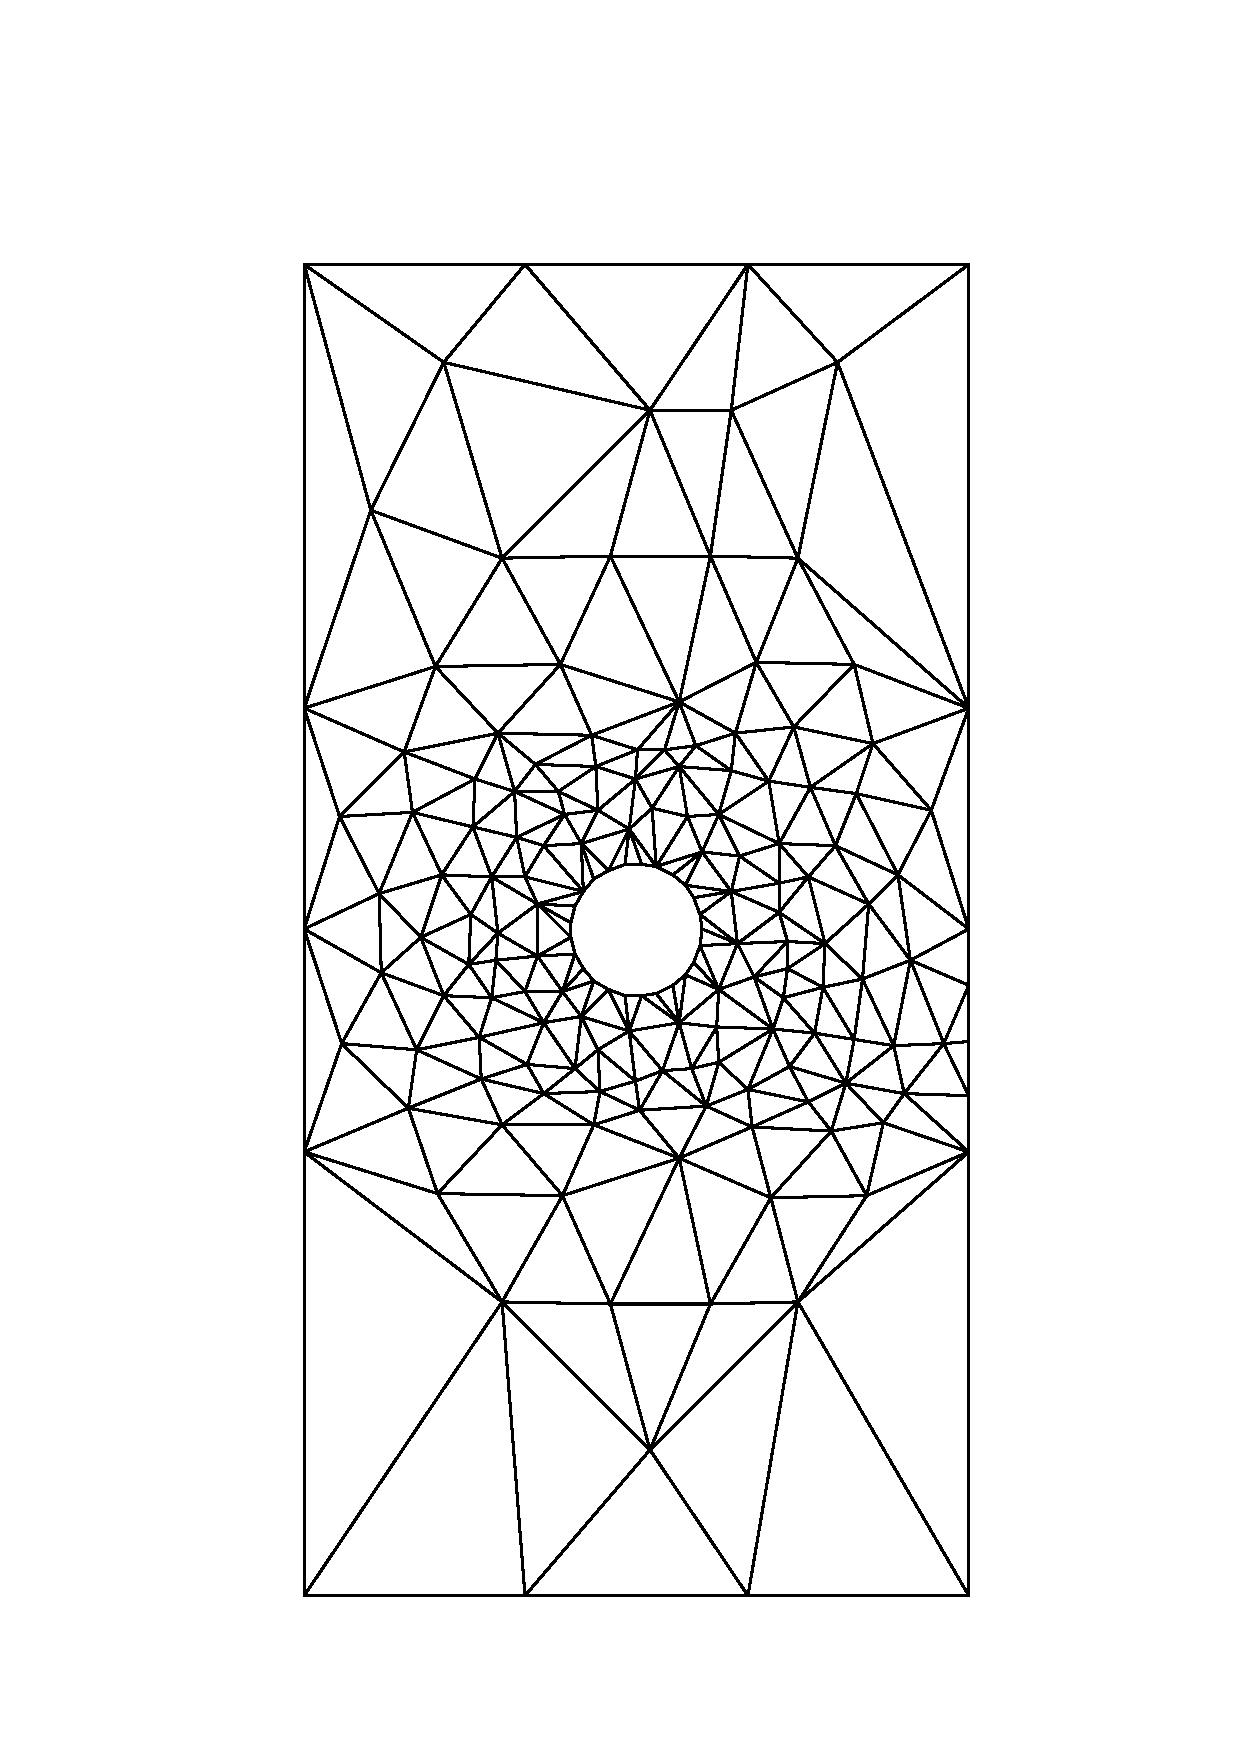
\includegraphics[height=.4\textwidth]{../plots/mesh3ele_u.pdf}\hspace{1cm}
	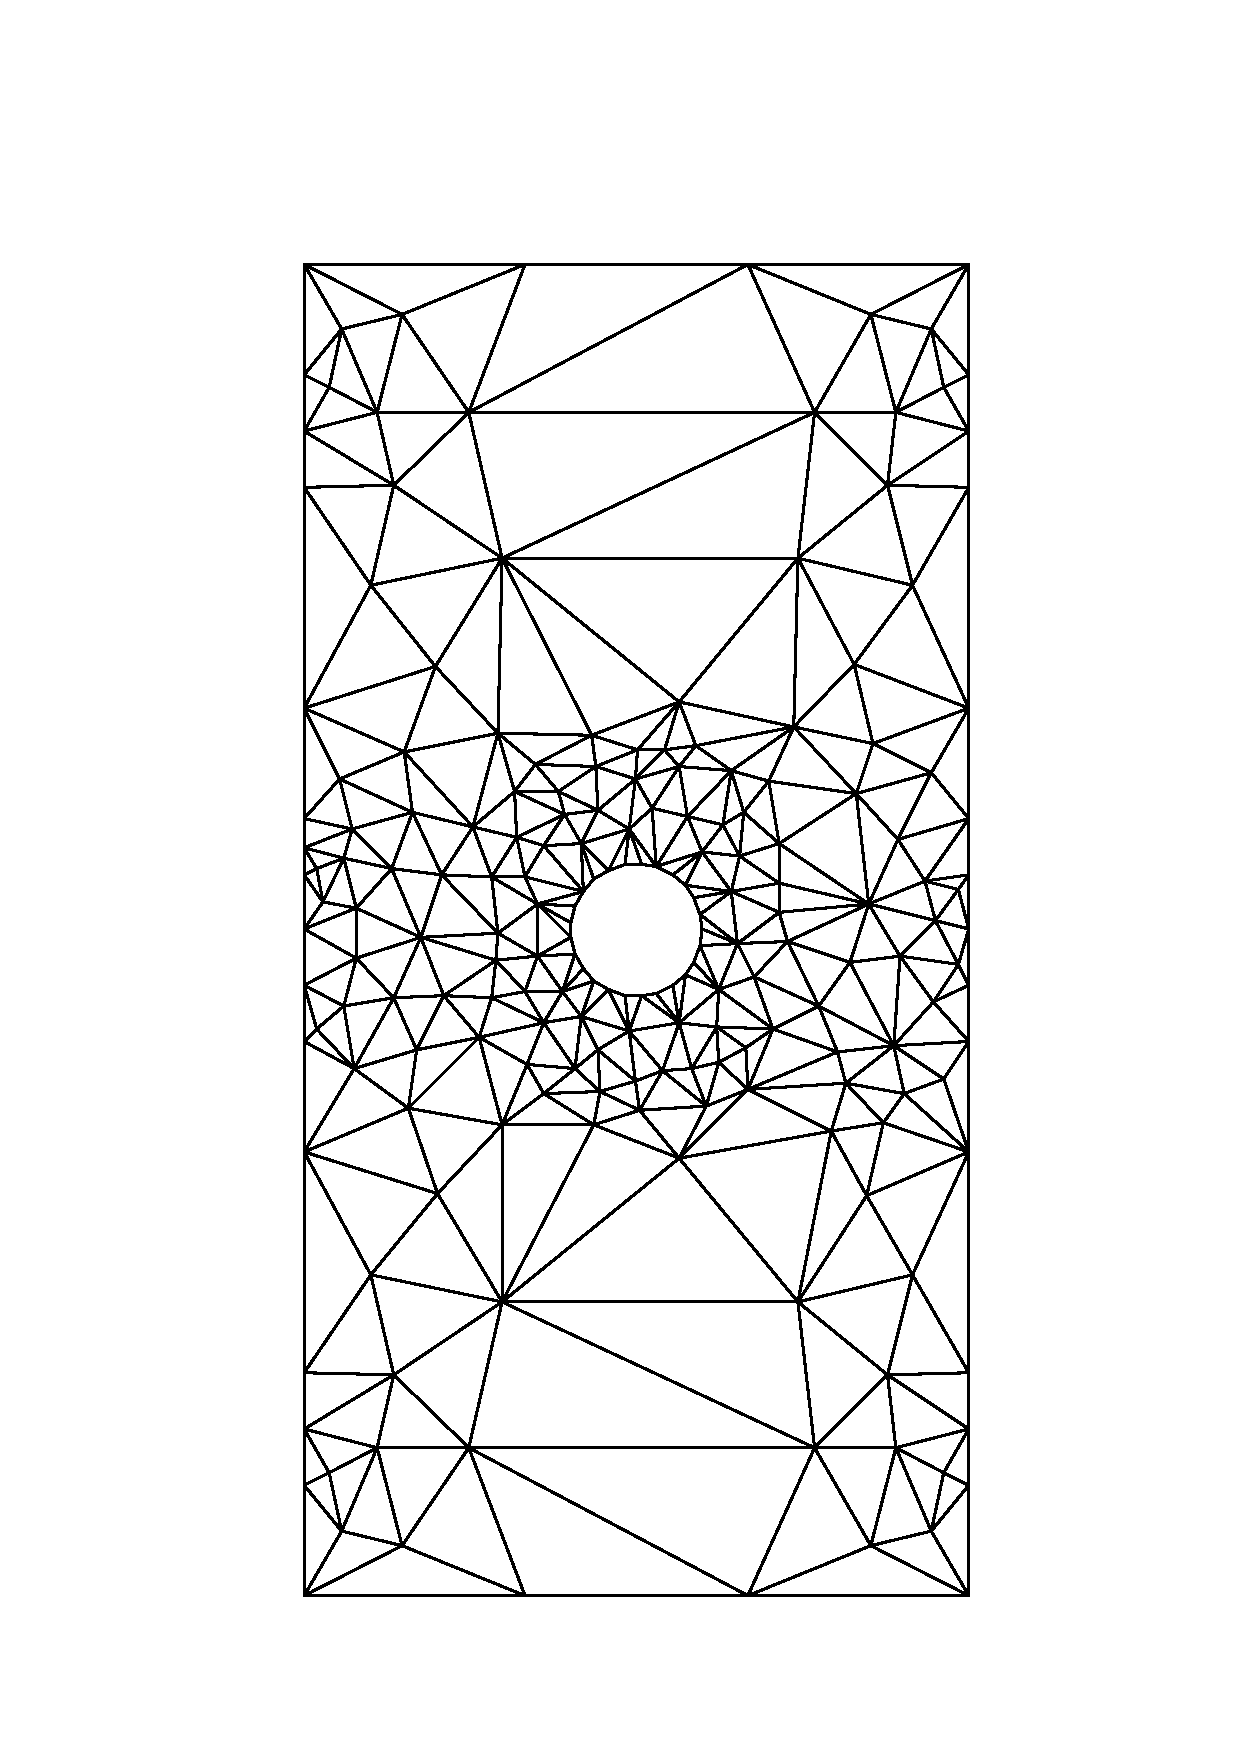
\includegraphics[height=.4\textwidth]{../plots/mesh3ele_v.pdf}\\~
}
\only<4>{
	Refinement 3\\~\\
	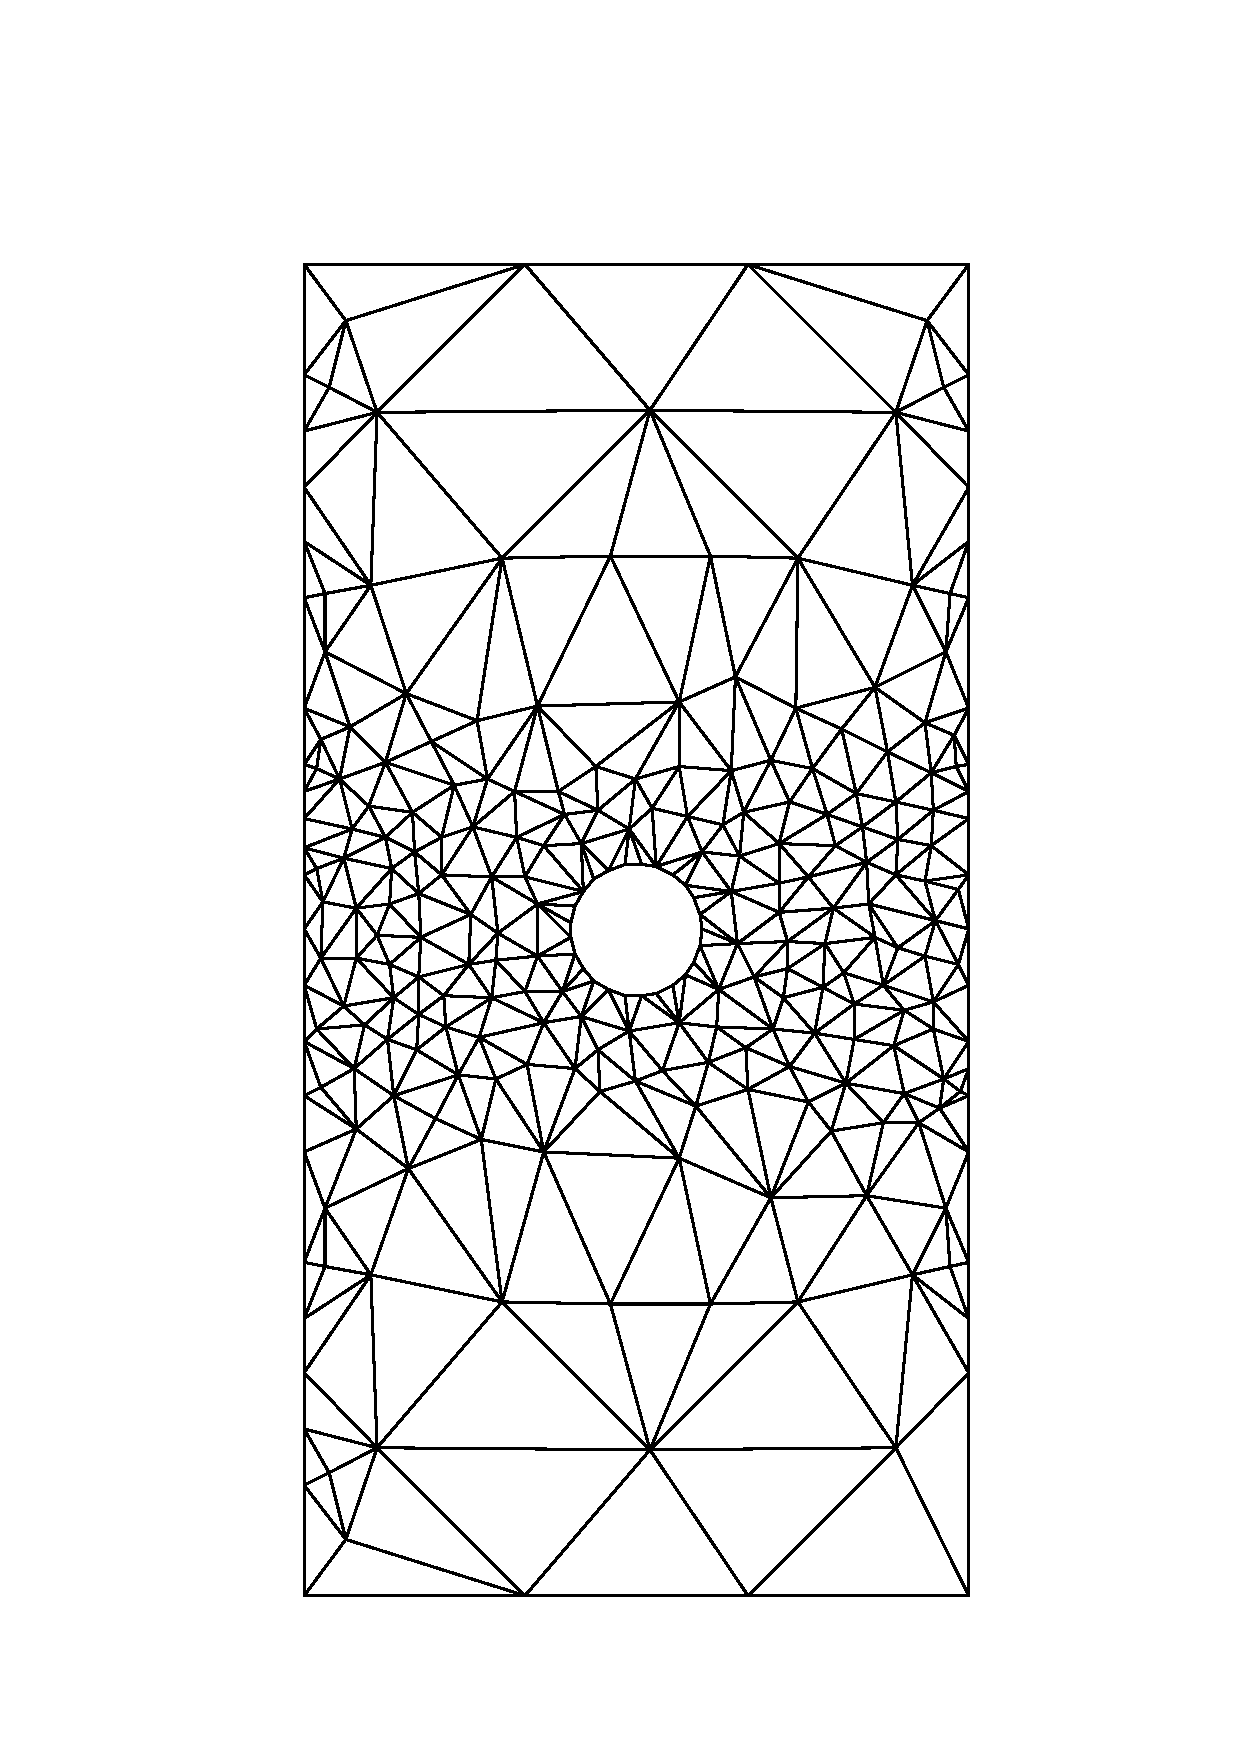
\includegraphics[height=.4\textwidth]{../plots/mesh4ele_p.pdf}\hspace{1cm}
	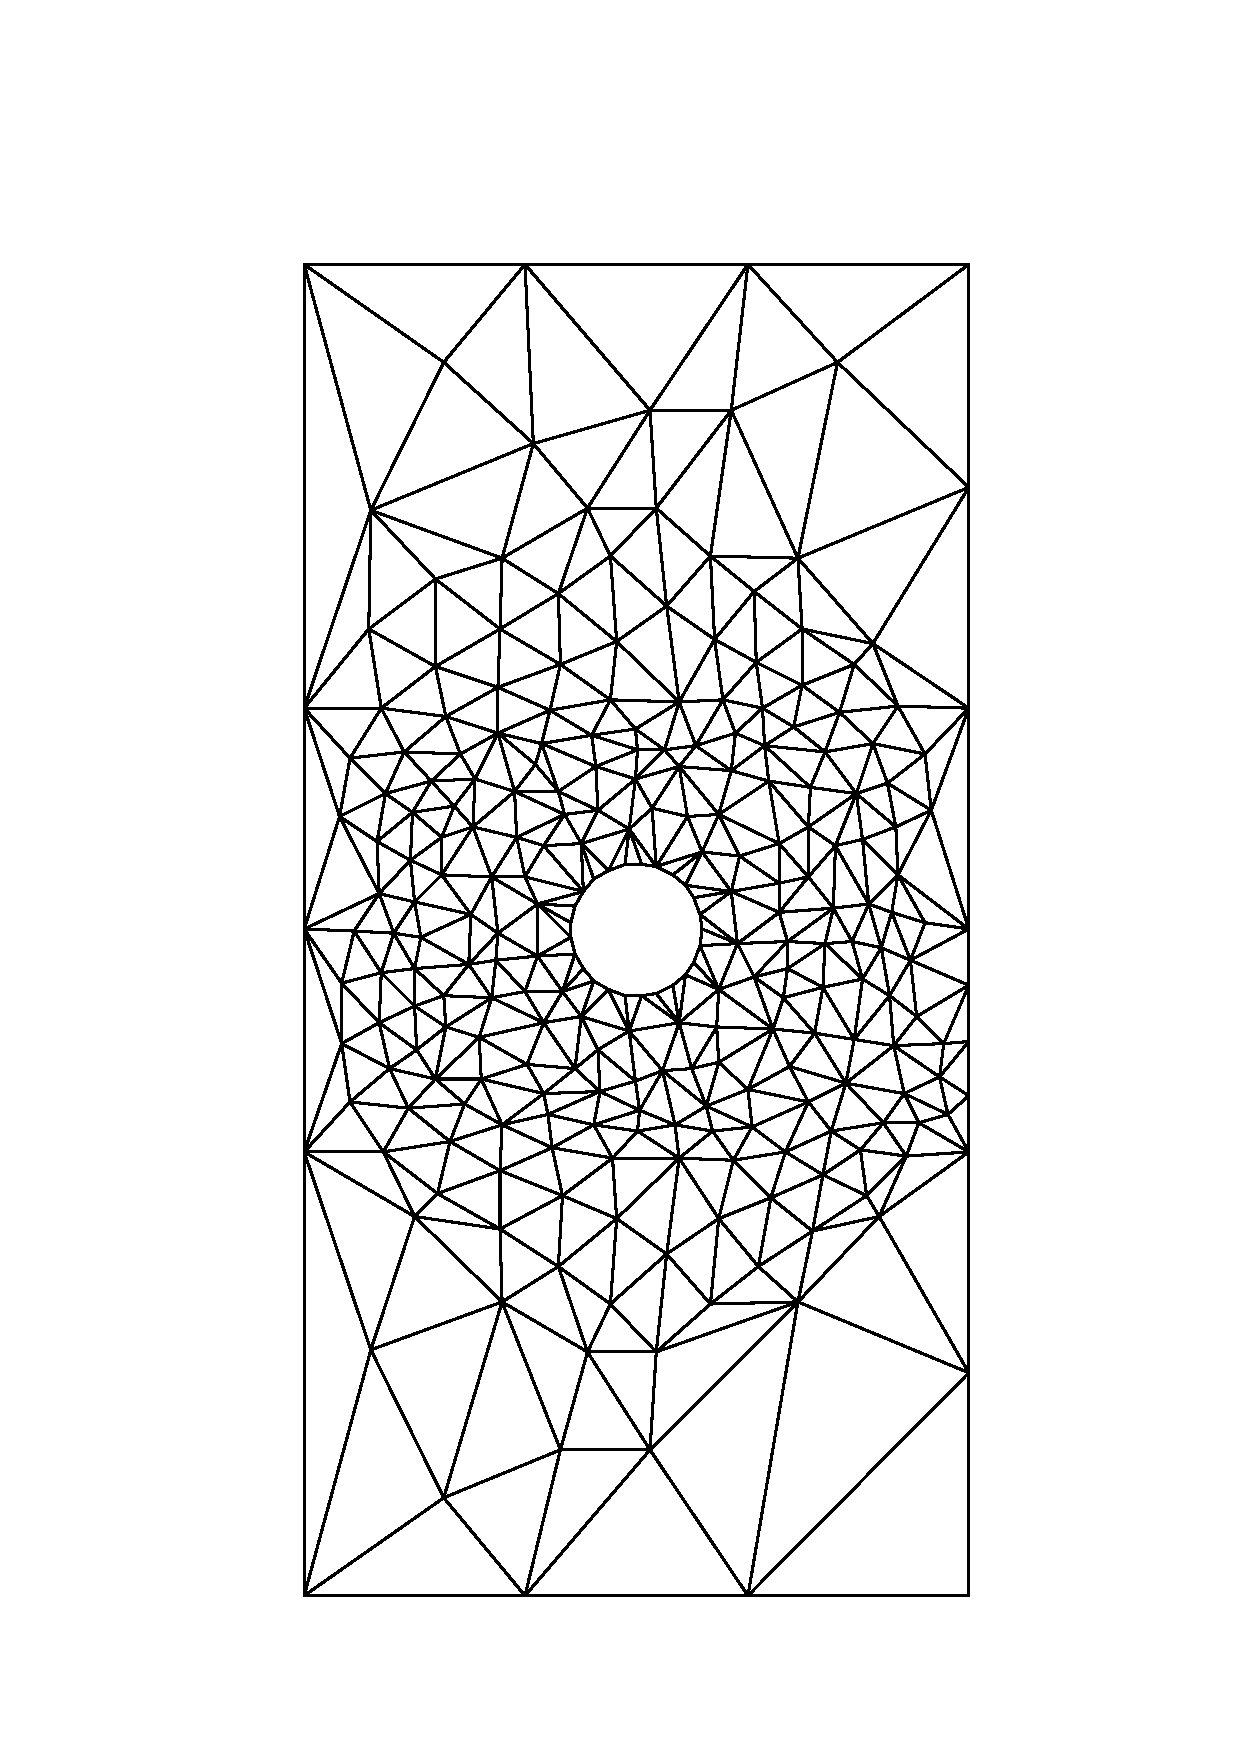
\includegraphics[height=.4\textwidth]{../plots/mesh4ele_u.pdf}\hspace{1cm}
	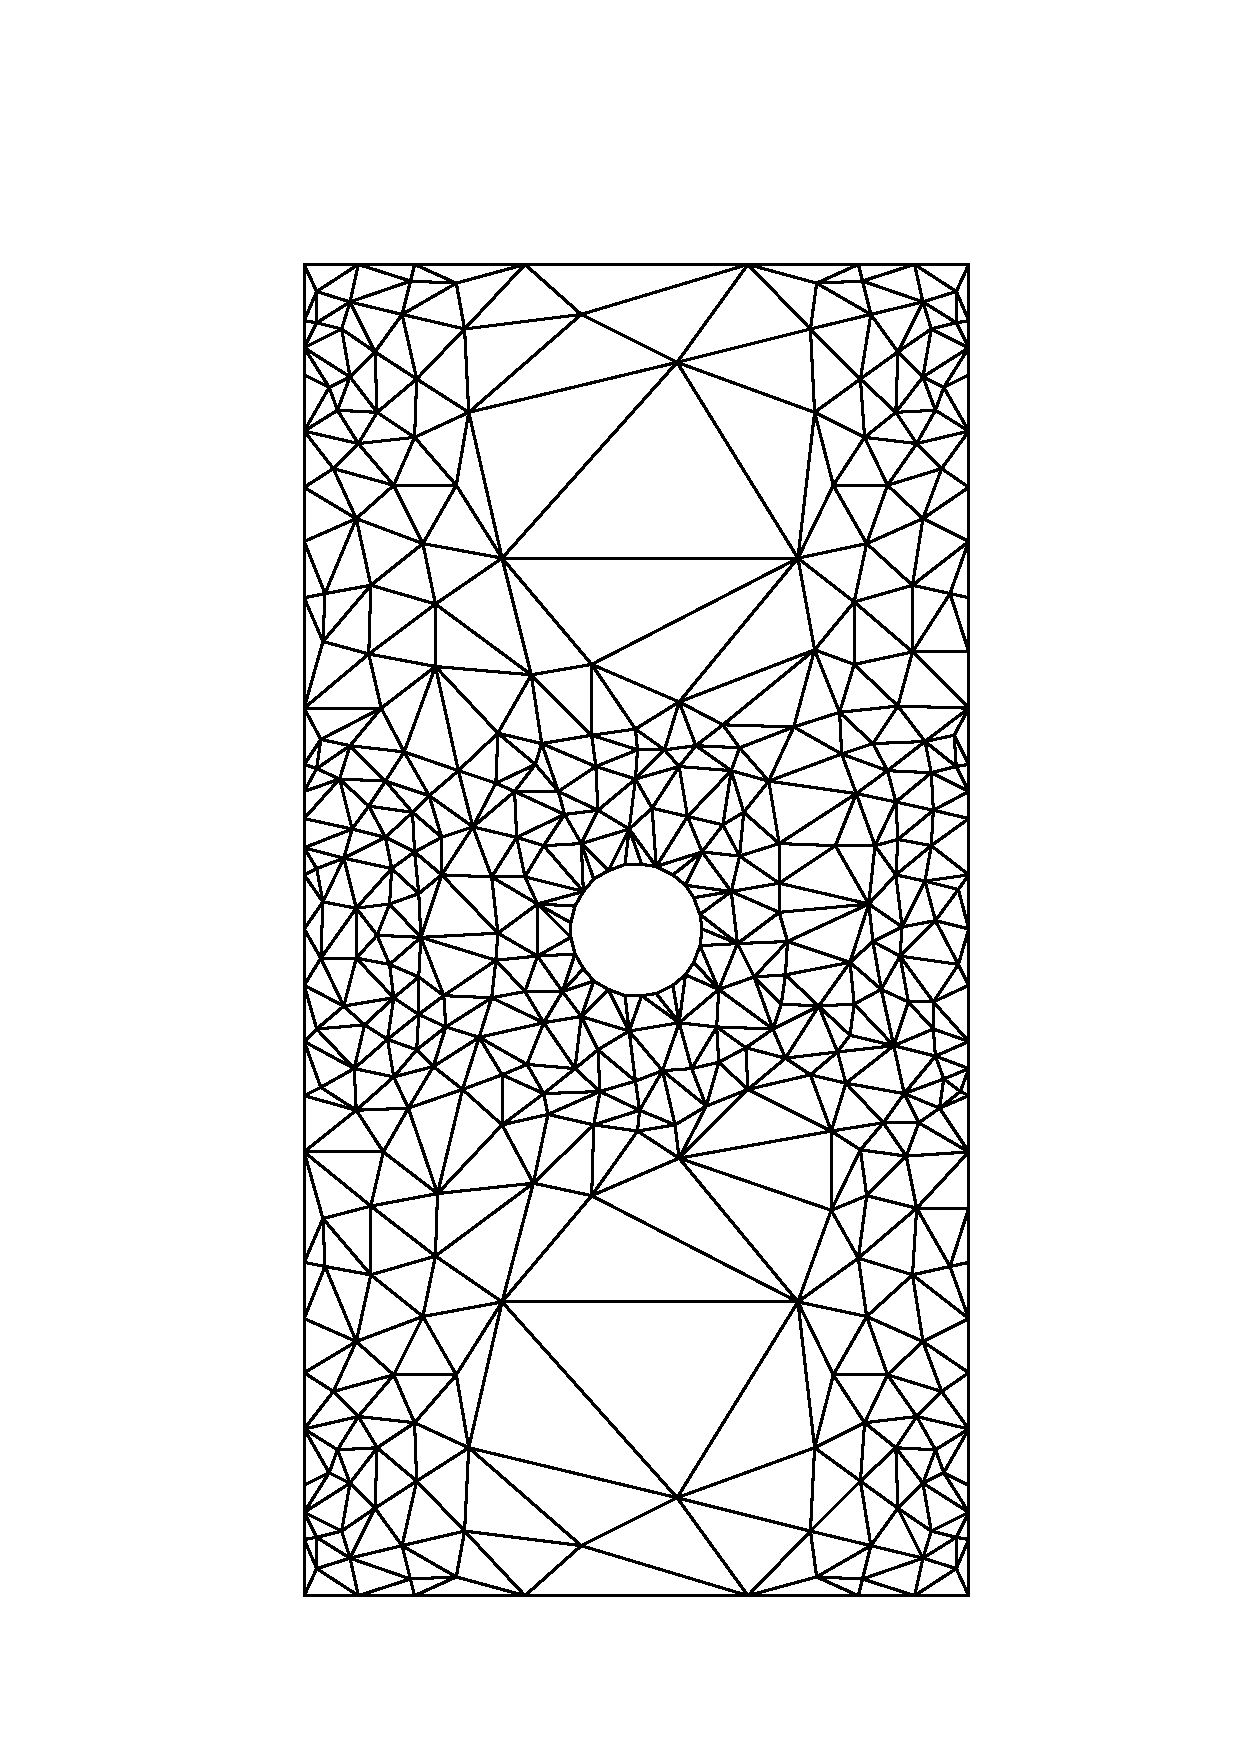
\includegraphics[height=.4\textwidth]{../plots/mesh4ele_v.pdf}\\
	{\hspace{1cm} Done}
}
\only<5>{
	Refinement 4\\~\\
	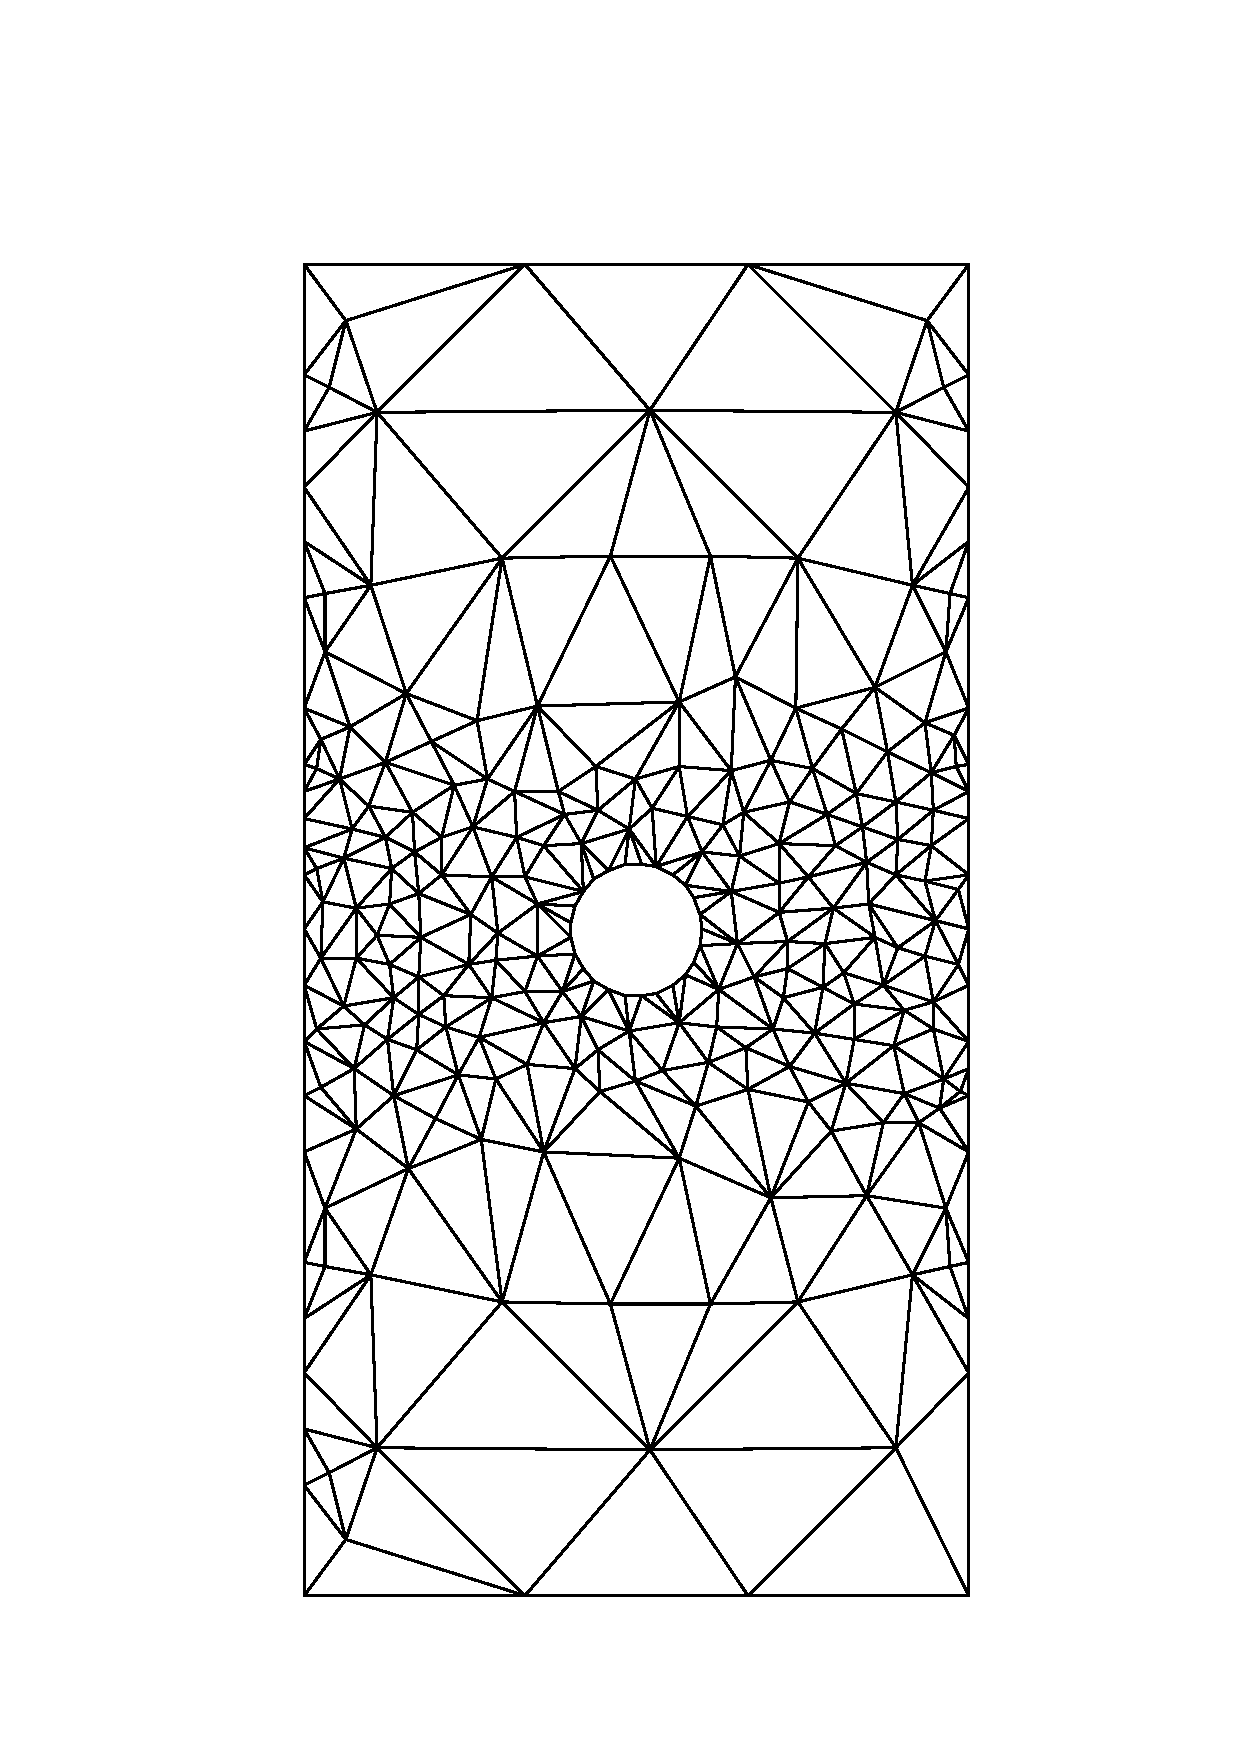
\includegraphics[height=.4\textwidth]{../plots/mesh4ele_p.pdf}\hspace{1cm}
	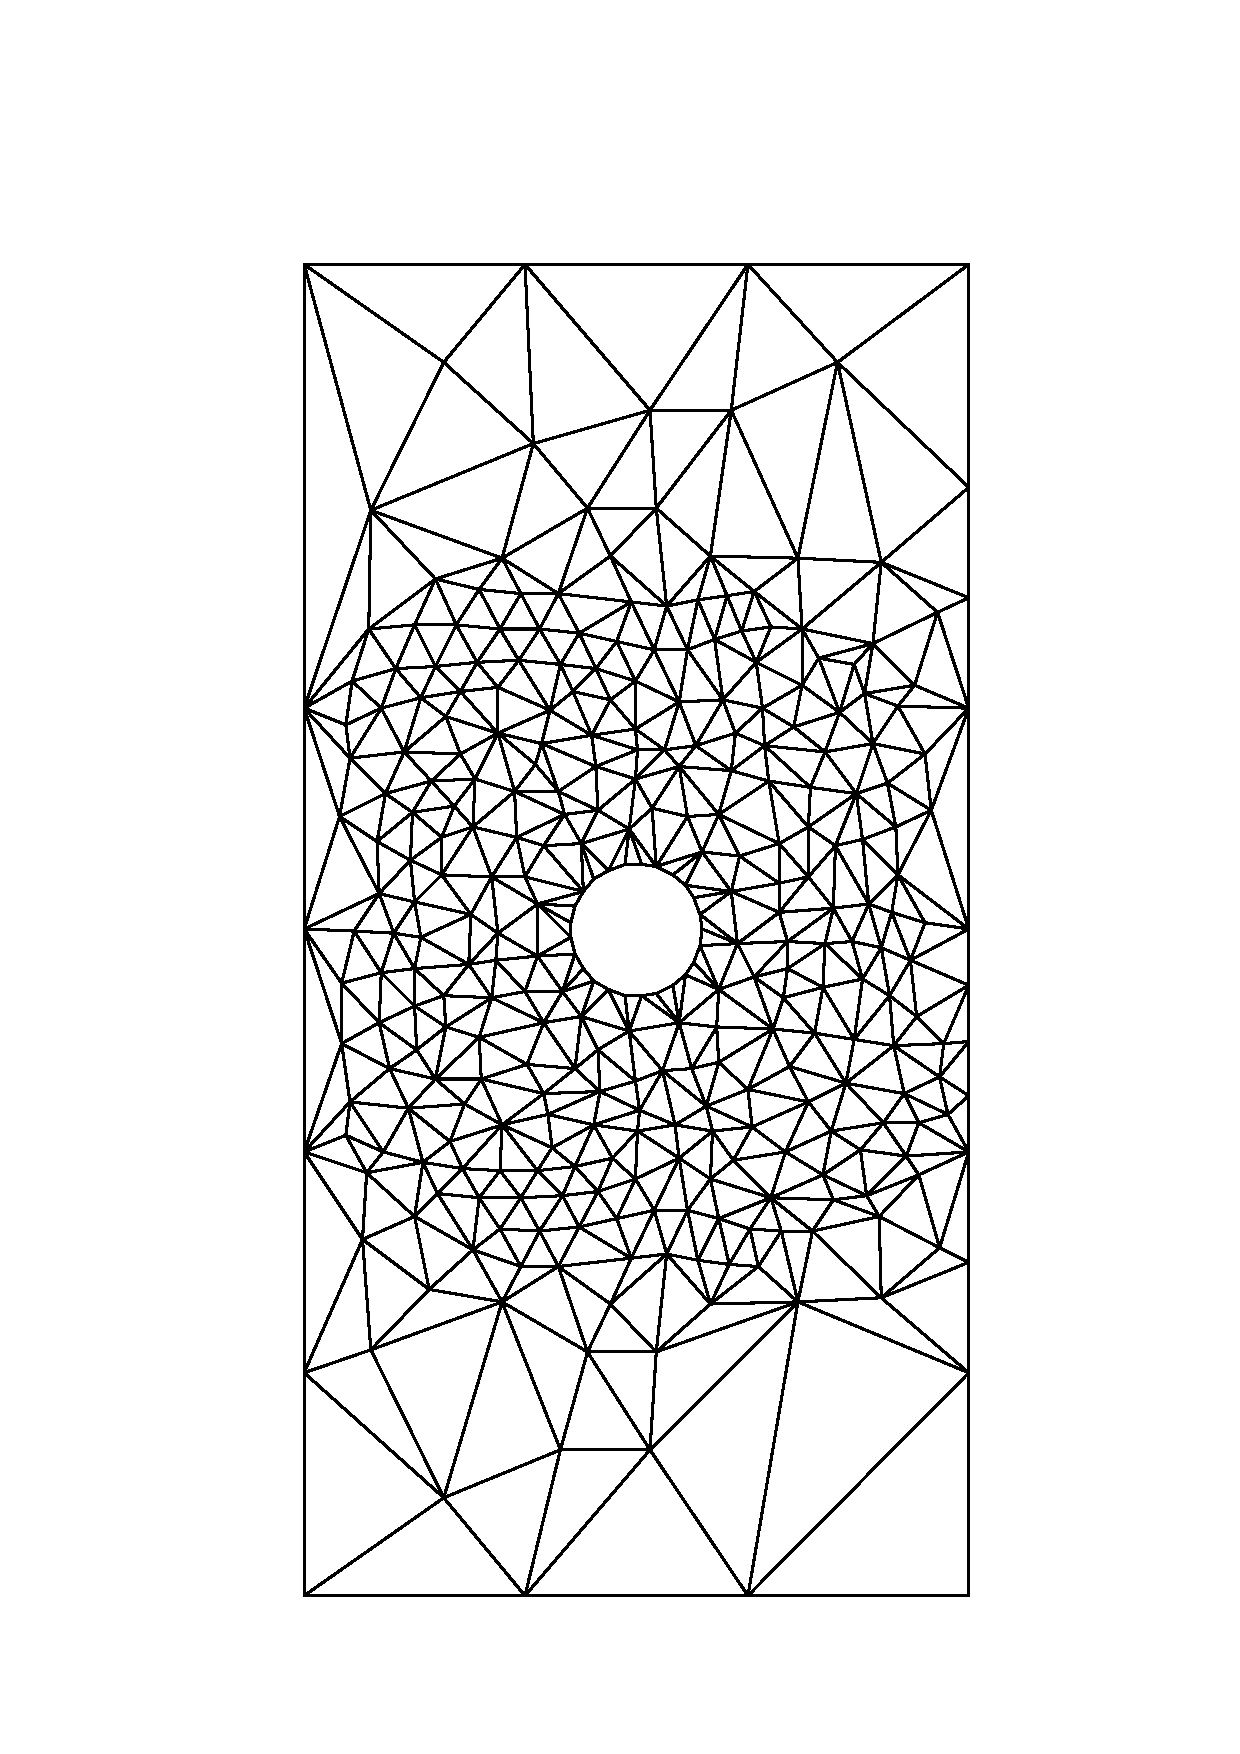
\includegraphics[height=.4\textwidth]{../plots/mesh5ele_u.pdf}\hspace{1cm}
	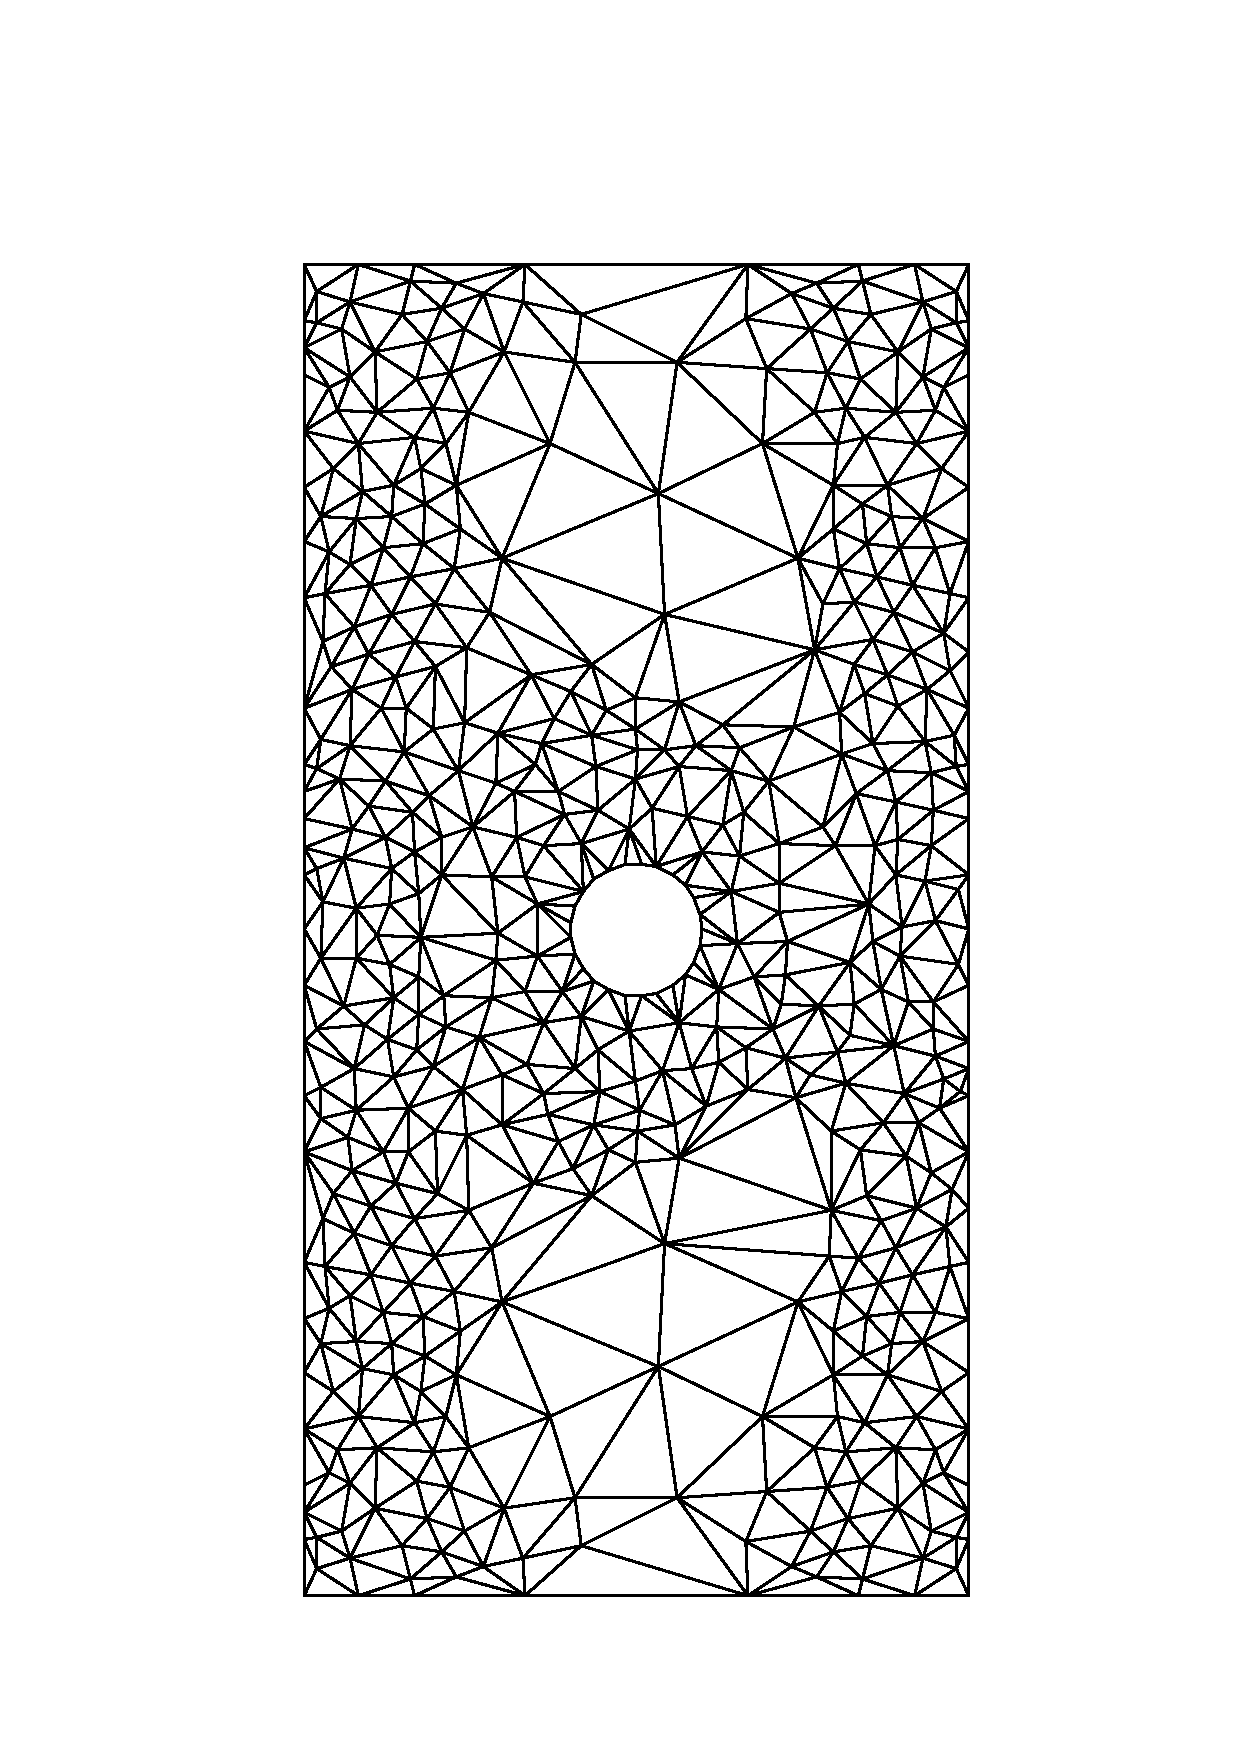
\includegraphics[height=.4\textwidth]{../plots/mesh5ele_v.pdf}\\
	{\hspace{1cm} Done}
}
\only<6>{
	Refinement 5\\~\\
	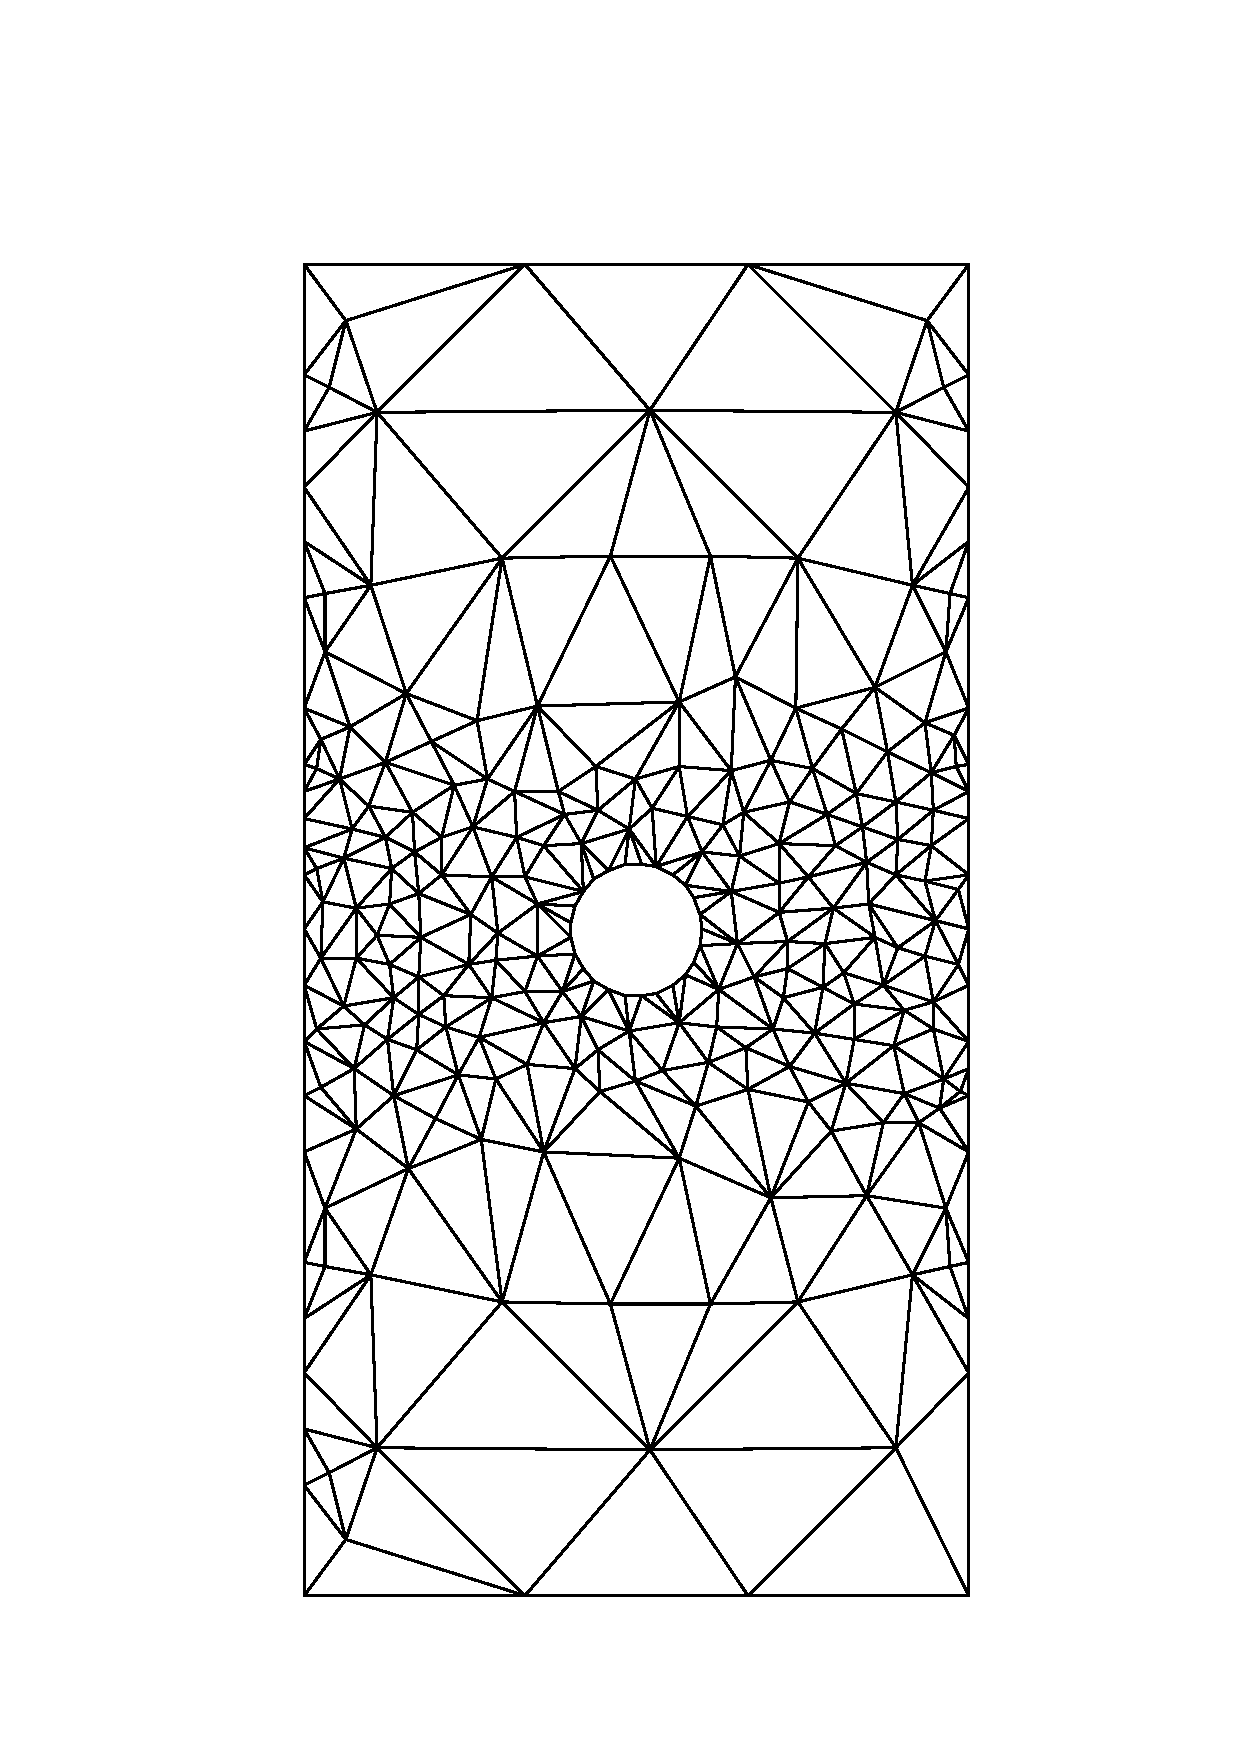
\includegraphics[height=.4\textwidth]{../plots/mesh4ele_p.pdf}\hspace{1cm}
	\includegraphics[height=.4\textwidth]{../plots/mesh6ele_u.pdf}\hspace{1cm}
	\includegraphics[height=.4\textwidth]{../plots/mesh6ele_v.pdf}\\
	{\hspace{1cm} Done \hspace{2cm} Done}
}
\only<7>{
	Refinement 6\\~\\
	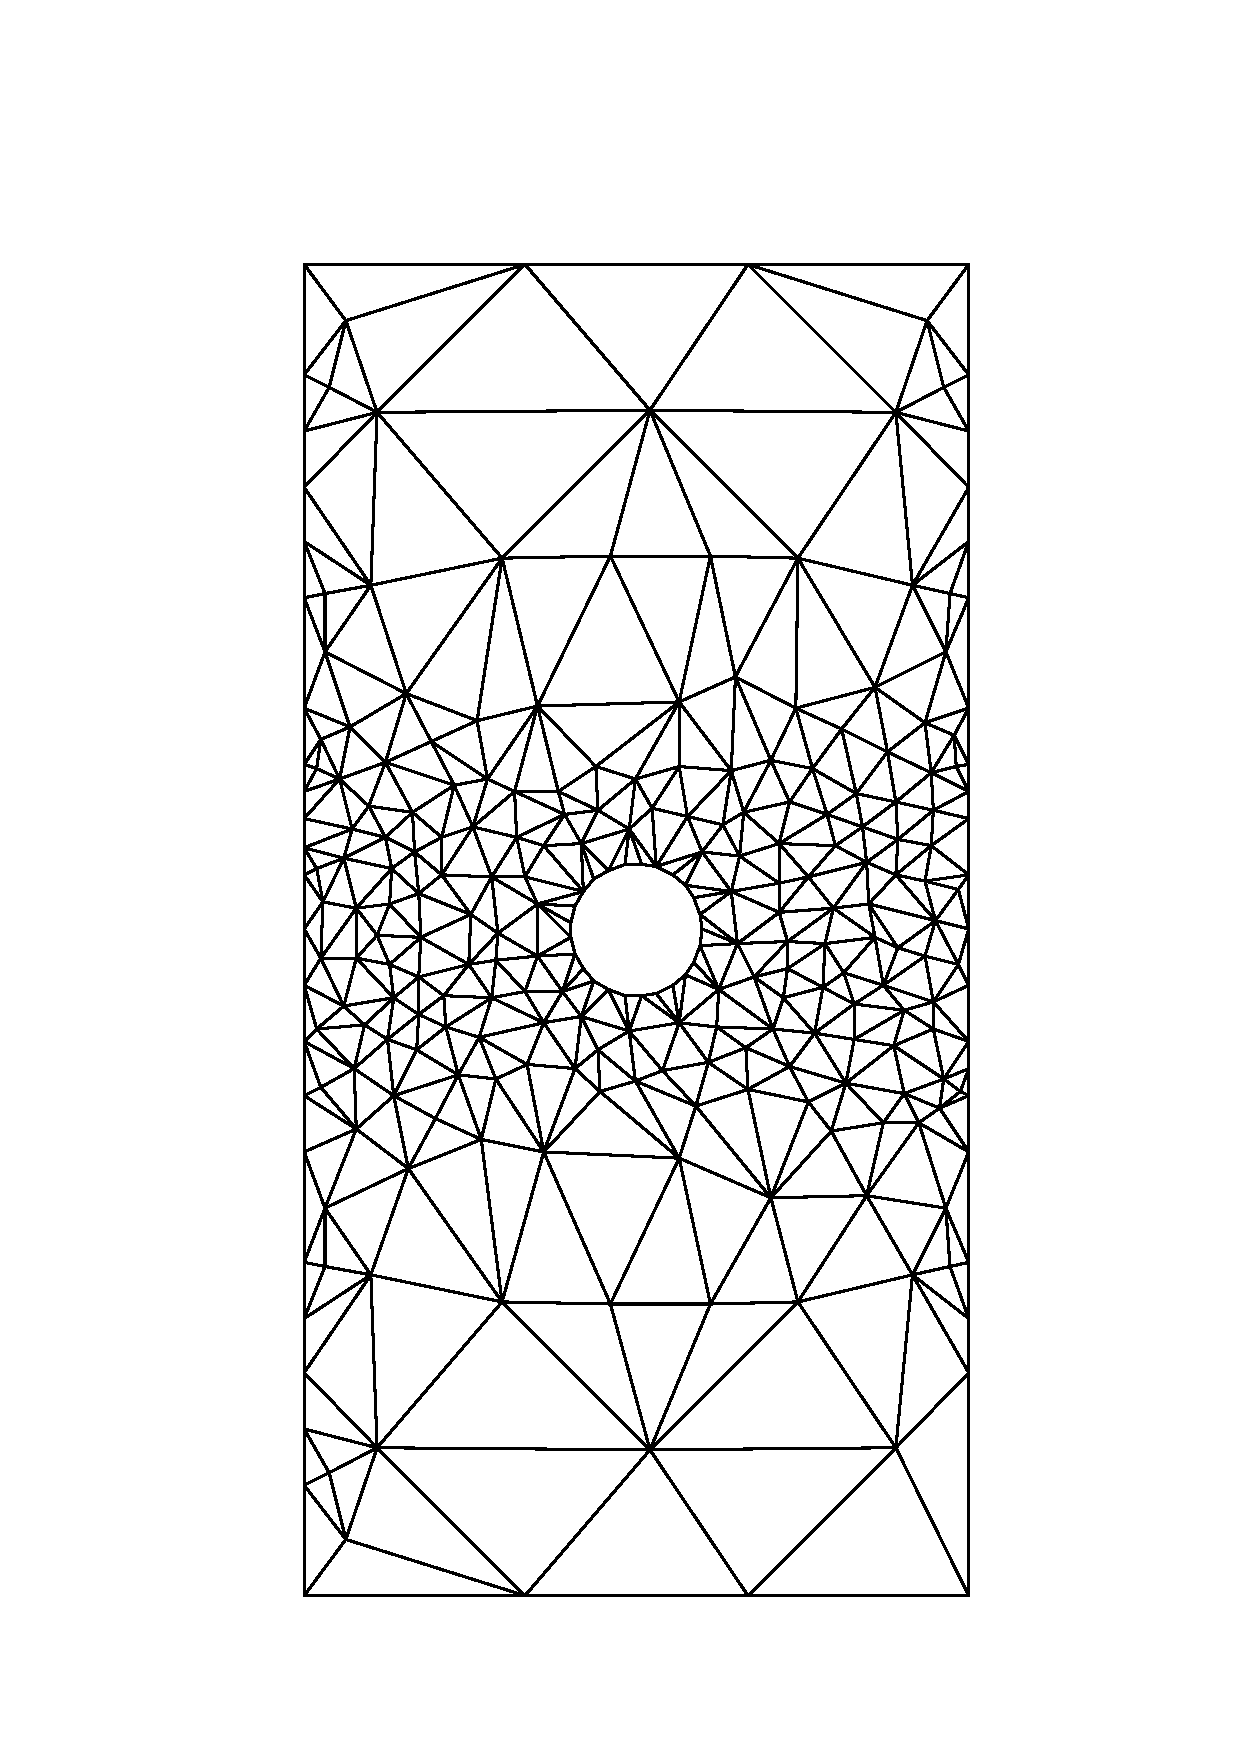
\includegraphics[height=.4\textwidth]{../plots/mesh4ele_p.pdf}\hspace{1cm}
	\includegraphics[height=.4\textwidth]{../plots/mesh6ele_u.pdf}\hspace{1cm}
	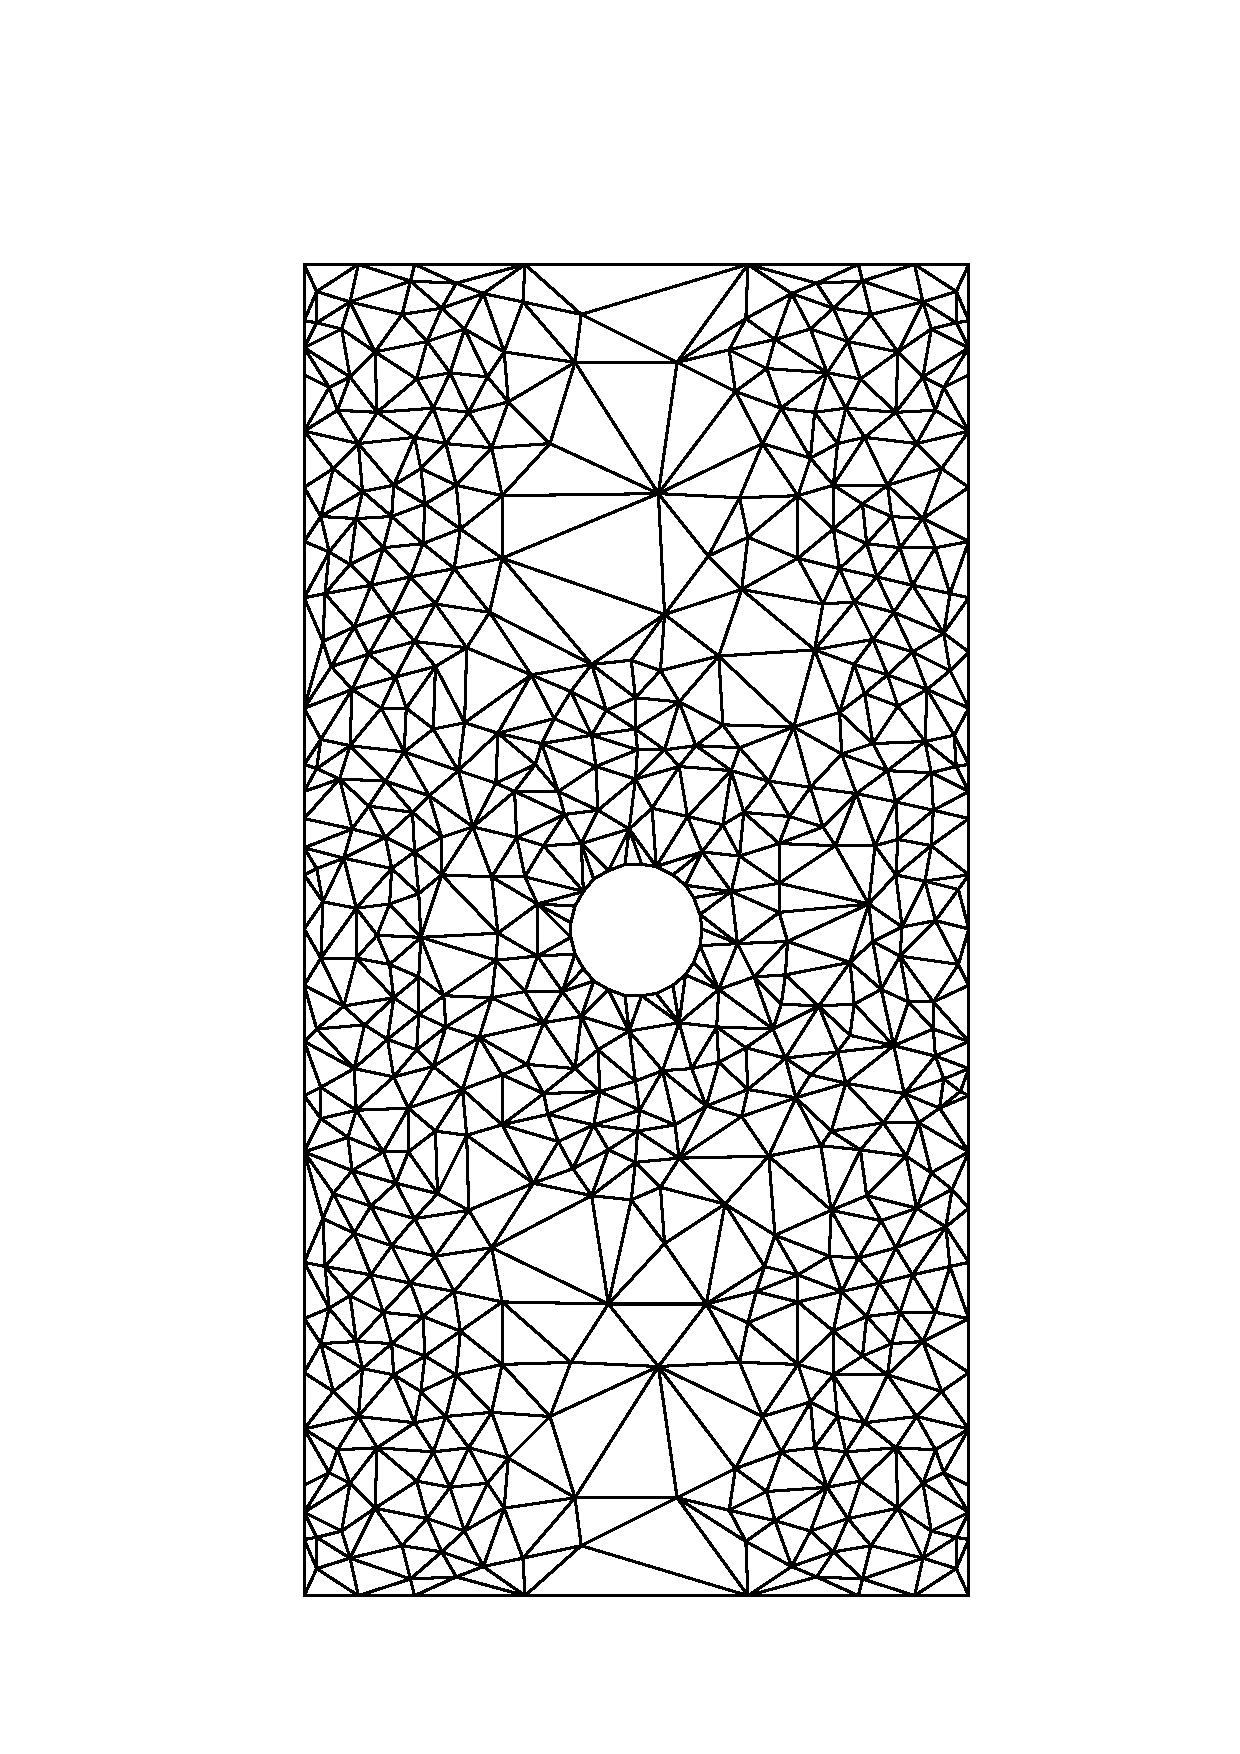
\includegraphics[height=.4\textwidth]{../plots/mesh7ele_v.pdf}\\
	{\hspace{1cm} Done \hspace{2cm} Done \hspace{2cm} Done}
}
\end{frame}

\subsection{5}
\begin{frame}%{Meshing Results}

\only<2>{{\tiny Pressure as error indicator\\}
\includegraphics[height=.25\textwidth]{../plots/p_5_row.pdf}}
\only<1-2>{\Large Meshing Results 5 Hole}\\
\only<2>{{\tiny Horizontal velocity as error indicator\\}
\includegraphics[height=.25\textwidth]{../plots/u_5_row.pdf}\\
{\tiny Vertical velocity as error indicator\\}
\includegraphics[height=.25\textwidth]{../plots/v_5_row.pdf}}
\end{frame}
%%%%%%%%%%%%%%%%%%%%%%%%%%%%%%%%%%%%%%

%%%%%%%%%%%%%%%%%%%%%%%%%%%%%%%%%%%%%
\subsection{13}
\begin{frame}%{Meshing Results}

{\tiny Pressure as error indicator\\}
\includegraphics[height=.25\textwidth]{../plots/p_13_row.pdf}
{\Large Meshing Results 13 Holes}\\
{\tiny Horizontal velocity as error indicator\\}
\includegraphics[height=.25\textwidth]{../plots/u_13_row.pdf}\\
{\tiny Vertical velocity as error indicator\\}
\includegraphics[height=.25\textwidth]{../plots/v_13_row.pdf}
\end{frame}

\subsection{Error Results}
\begin{frame}%{Error Results}

\includegraphics[width=.4\textwidth]{../plots/errorstep_1.pdf}
\includegraphics[width=.4\textwidth]{../plots/errorstep_5.pdf}\\
\hspace{1cm}1 Obstruction \hspace{1.6cm} 5 Obstructions
\includegraphics[width=.4\textwidth]{../plots/errorstep_13.pdf}
\tikz{\draw[help lines,white] (-1,-.5) grid (1,.5);
\pgftext[bottom,at={\pgfpoint{2cm}{1.5cm}}]{{\Large Error Results}}}
\\
%\hspace{3cm} 
13 Obstructions
\end{frame}

\section{Computation Time Results}
\subsection{LAPACK vs. SLAP}
\begin{frame}{Computation Time Results - Sparse vs. Dense Solvers}
\pause
\includegraphics[width=.48\textwidth]{../plots/sparse_small.pdf}\pause
\includegraphics[width=.5\textwidth]{../plots/solution_times.pdf}\\
{\hspace{1cm}Sparseness \hspace{3.5cm} Computation Time}

\end{frame}
\section{Conclusions}
\subsection{Conclusions}
\begin{frame}{Conclusions}
\begin{itemize}
\item Reproduced well know flow patterns around cylinders at very low Reynolds numbers.
\item Implemented unstructured adaptive meshing algorithm.
	\begin{itemize}
	\item Pressure performed well as an error indicator
	\item Different Error indicators produced very different meshes.  
	\end{itemize}
\item Sparse matrix storage and equation solver drastically reduced solution time.  
\end{itemize}
\end{frame}
\end{document}  